\documentclass[11pt,a4paper]{article}

\usepackage[margin=2.5cm]{geometry}
\usepackage{amsmath,amssymb}
\usepackage{graphicx}
\usepackage{booktabs}
\usepackage{caption}
\usepackage{float}
\usepackage[hidelinks]{hyperref}
\usepackage{microtype}
\usepackage{enumitem}

\captionsetup{font=small,labelfont=bf}
\setlength{\parskip}{0.4em}
\setlength{\parindent}{0pt}

\newcommand{\code}[1]{\texttt{#1}}

\title{\vspace{-1.5cm}Statistical Learning and Data Analytics for Transportation Systems\\[0.3em]
\large Problem Set 2 --- Dimensionality Reduction, Logistic Regression,\\
Support Vector Machines, Decision Trees and Ensemble Learning}
\author{Mohd Zamin Quadri}
\date{July 2026}

\begin{document}
\maketitle

\vspace{-0.8em}
\noindent\rule{\textwidth}{0.4pt}

All computations, figures and tables in this report were produced by the accompanying
notebook \code{Problem\_Set\_2\_Notebook.ipynb}, which is submitted with its outputs. Every
number quoted below is taken from an executed cell of that notebook; nothing has been
computed by hand and transcribed. Figures are reproduced here from the \code{figures/}
folder and the underlying tables are also written to \code{results/} as CSV files.

\vspace{0.3em}
\noindent\rule{\textwidth}{0.4pt}

% =====================================================================
\section{Problem 1 (35 points)}

The dependent variable is the observed travel mode, coded $0$ for walking and $1$ for
travel by car. Both models are binomial logistic regressions, so for respondent $i$
\begin{equation}
\Pr(\text{car}_i = 1 \mid \mathbf{x}_i) = \frac{1}{1 + e^{-\eta_i}},
\qquad
\eta_i = \beta_0 + \sum_{j=1}^{K}\beta_j x_{ij},
\label{eq:logit}
\end{equation}
where $\eta_i$ is the linear predictor and $e^{\eta_i}$ are the odds of choosing the car.
Model 1 contains five regressors (\code{TrvlTime}, \code{Age},
\code{Indiv\_trvl\_frequency}, \code{HHVeh}, \code{HHsize}); Model 2 is Model 1 with
\code{Indiv\_trvl\_frequency} removed. Both were estimated on the same $n = 244{,}493$
observations, so the models are nested and directly comparable.

% ---------------------------------------------------------------------
\subsection{Performance of the two models (10 points)}

\paragraph{Method.} Because the models are nested and share the same sample, two
complementary comparisons are available. The first is the penalised likelihood. The
Bayesian information criterion is
\begin{equation}
\mathrm{BIC} = -2\ln\hat{L} + k\ln n,
\label{eq:bic}
\end{equation}
where $k$ counts all estimated parameters including the intercept. Since the reported BIC
values were computed on identical data, they can be compared directly, and
Equation~\eqref{eq:bic} can also be inverted to recover the maximised log-likelihood of
each model. The second comparison is a likelihood-ratio test of the restriction that the
dropped variable has no effect,
\begin{equation}
H_0:\ \beta_{\text{Indiv\_trvl\_frequency}} = 0,
\qquad
\Lambda = 2\left(\ln\hat{L}_1 - \ln\hat{L}_2\right) \overset{H_0}{\sim} \chi^2_1 .
\label{eq:lr}
\end{equation}
Note that an $R^2$ is not defined for a logistic model in the way it is for the linear
models of Problem Set 1, which is why the comparison rests on the likelihood rather than
on explained variance.

\paragraph{Results.} With $\ln n = 12.406942$, inverting Equation~\eqref{eq:bic} gives the
figures in Table~\ref{tab:fit}.

\begin{table}[H]
\centering
\caption{Fit statistics for the two models ($n = 244{,}493$).}
\label{tab:fit}
\begin{tabular}{lrrrr}
\toprule
& $k$ & BIC (reported) & $\ln\hat{L}$ (recovered) & AIC \\
\midrule
Model 1 & 6 & 95{,}815.66 & $-47{,}870.609$ & 95{,}753.218 \\
Model 2 & 5 & 97{,}047.60 & $-48{,}492.783$ & 96{,}995.565 \\
\midrule
Difference (Model 2 $-$ Model 1) & & $+1231.94$ & $-622.174$ & $+1242.35$ \\
\bottomrule
\end{tabular}
\end{table}

The likelihood-ratio statistic of Equation~\eqref{eq:lr} is
$\Lambda = 1244.35$ on 1 degree of freedom, with $p = 1.4 \times 10^{-272}$.

Every parameter in both models is significant at any conventional level: the smallest
$|z|$ anywhere is $2.888$ for \code{HHsize} in Model 2, which still gives $p = 0.0039$.
Significance alone therefore cannot separate the two models. Table~\ref{tab:shift} shows
what happens to the coefficients that both models share.

\begin{table}[H]
\centering
\caption{Coefficients common to both models, and the effect of dropping
\code{Indiv\_trvl\_frequency}.}
\label{tab:shift}
\begin{tabular}{lrrrrr}
\toprule
Variable & Model 1 & Model 2 & $|z|$ Model 1 & $|z|$ Model 2 & Change (\%) \\
\midrule
(Intercept)        & $-2.1260$ & $-2.0380$ & 78.723  & 75.778  & $+4.14$ \\
\code{TrvlTime}    & $0.000979$ & $0.000947$ & 94.334  & 92.282  & $-3.28$ \\
\code{Age}         & $0.01716$ & $0.01711$ & 44.485  & 44.149  & $-0.29$ \\
\code{HHVeh}       & $1.0120$  & $1.1880$  & 113.359 & 157.549 & $+17.39$ \\
\code{HHsize}      & $-0.02463$ & $-0.00937$ & 7.497   & 2.888   & $+61.97$ \\
\bottomrule
\end{tabular}
\end{table}

\paragraph{Interpretation.} \textbf{Model 1 is the better model.} Three separate arguments
point the same way.

First, the penalised likelihood. Model 1 has the lower BIC by 1231.94 points. On the usual
Kass--Raftery reading, a BIC difference above 10 already constitutes decisive evidence, so
a gap of more than a thousand leaves no room for doubt. The AIC, which penalises
complexity more weakly, agrees by an even larger margin. It is worth being explicit that
BIC already contains a penalty for the extra parameter --- Model 1 wins \emph{despite}
being the larger model, so the usual appeal to parsimony does not rescue Model 2.

Second, the likelihood-ratio test. Adding \code{Indiv\_trvl\_frequency} buys 622.17
log-likelihood points for a single degree of freedom, which is overwhelming evidence
against the restriction.

Third, and most important for interpretation, Model 2's remaining parameters are highly
sensitive to the exclusion. \code{HHVeh} inflates by 17\% from 1.012 to 1.188, and
\code{HHsize} shrinks by about 62\% with its $|z|$ falling from 7.50 to 2.89.

Two mechanisms could produce this, and the printed output alone cannot separate them. The
first is \emph{omitted-variable bias}: the dropped variable is positively correlated with
\code{HHVeh} in the sample examined in Section~\ref{sec:pca} ($r = 0.609$), so the vehicle
coefficient can absorb part of its effect. The second is \emph{non-collapsibility}, a
feature specific to non-linear link functions: in a logistic model, omitting any covariate
that predicts the outcome changes the remaining coefficients even when the omitted variable
is uncorrelated with those retained. I therefore describe the changes as \emph{consistent
with} omitted-variable bias or non-collapsibility rather than asserting bias outright, and
I do not claim that Model 1's parameters are unbiased --- Model 1 may itself omit relevant
variables such as income, licence holding or residential density, none of which are
available here.

Two further cautions. The correlation of $0.609$ is measured on the 5000-row sample of
Section~\ref{sec:pca}, whereas the models are estimated on 244,493 observations, so it is
indicative rather than a direct measurement on the estimation sample. And \code{HHsize}
remains statistically significant in Model 2 ($p = 0.0039$, significant at the 1\% level);
what falls sharply is its estimated magnitude and precision, not its significance.

The signs in Model 1 are all consistent with travel behaviour. Longer trips favour the car
over walking, which is expected since walking becomes impractical as distance grows. Older
travellers and more frequent travellers are more likely to drive. Household vehicle
ownership has by far the strongest effect, with an odds ratio of $e^{1.012} = 2.751$ per
additional vehicle. Larger households are slightly less likely to travel by car
($e^{-0.02463} = 0.976$ per additional person), plausibly because a fixed vehicle fleet is
shared among more people. Because the coefficient on \code{TrvlTime} is expressed per
second it looks negligible, but scaled to a realistic increment it is substantial: an
extra ten minutes of travel time multiplies the odds of driving by
$e^{0.000979 \times 600} = 1.799$.

\paragraph{Assumption and limitation.} One caveat should be stated clearly. BIC and the
likelihood-ratio test both measure how well a model fits the data in the likelihood sense.
The question asks which model is best \emph{for classifying} travel mode, and likelihood
fit is not the same thing as classification accuracy. A proper answer to the classification
question would require a held-out sample and metrics such as accuracy, recall or the area
under the ROC curve, none of which can be computed from the printed output supplied. What
can be said with confidence is that Model 1 describes the data substantially better in the
likelihood sense and therefore provides the stronger statistical basis for classification.
Neither unbiasedness of its parameters nor its held-out classification performance can be
established from the output supplied. The strength of the evidence is also inflated by the
sample size: with $n = 244{,}493$, even a small effect will be highly significant, so the
magnitude of the effects matters more than their $p$-values.

% ---------------------------------------------------------------------
\subsection{Predicted probability of choosing the car (15 points)}

\paragraph{Method.} Model 1 was identified as the better model, so its coefficients are
used. For each respondent the linear predictor is formed and passed through the logistic
link of Equation~\eqref{eq:logit}:
\[
\eta = \hat\beta_0
     + \hat\beta_1 \code{TrvlTime}
     + \hat\beta_2 \code{Age}
     + \hat\beta_3 \code{Indiv\_trvl\_frequency}
     + \hat\beta_4 \code{HHVeh}
     + \hat\beta_5 \code{HHsize} .
\]
Table~\ref{tab:contrib} shows each term separately so that the arithmetic is visible.

\begin{table}[H]
\centering
\caption{Contribution of each term to the linear predictor, and the resulting probability.
\code{TrvlTime} is in seconds.}
\label{tab:contrib}
\begin{tabular}{lrrrrrrrr}
\toprule
& Intercept & \code{TrvlTime} & \code{Age} & \code{Ind.freq} & \code{HHVeh} &
\code{HHsize} & $\eta$ & $\hat P(\text{car})$ \\
\midrule
A & $-2.1260$ & $3.5719$ & $1.0296$ & $0.3866$ & $2.0240$ & $-0.0493$ & $4.8369$ & $0.9921$ \\
B & $-2.1260$ & $0.1957$ & $0.4462$ & $0.1128$ & $0.0000$ & $-0.0246$ & $-1.3960$ & $0.1985$ \\
\bottomrule
\end{tabular}
\end{table}

\paragraph{Results.}
\begin{align*}
\text{Respondent A:}\quad &\eta_A = 4.8369, \quad
\text{odds} = e^{4.8369} = 126.074, \quad
\hat P(\text{car}) = \frac{1}{1+e^{-4.8369}} = \mathbf{0.9921}, \\
\text{Respondent B:}\quad &\eta_B = -1.3960, \quad
\text{odds} = e^{-1.3960} = 0.2476, \quad
\hat P(\text{car}) = \frac{1}{1+e^{1.3960}} = \mathbf{0.1985}.
\end{align*}
So respondent A is predicted to travel by car with probability $0.992$
($\hat P(\text{walk}) = 0.008$) and respondent B with probability $0.198$
($\hat P(\text{walk}) = 0.802$).

\begin{figure}[H]
\centering
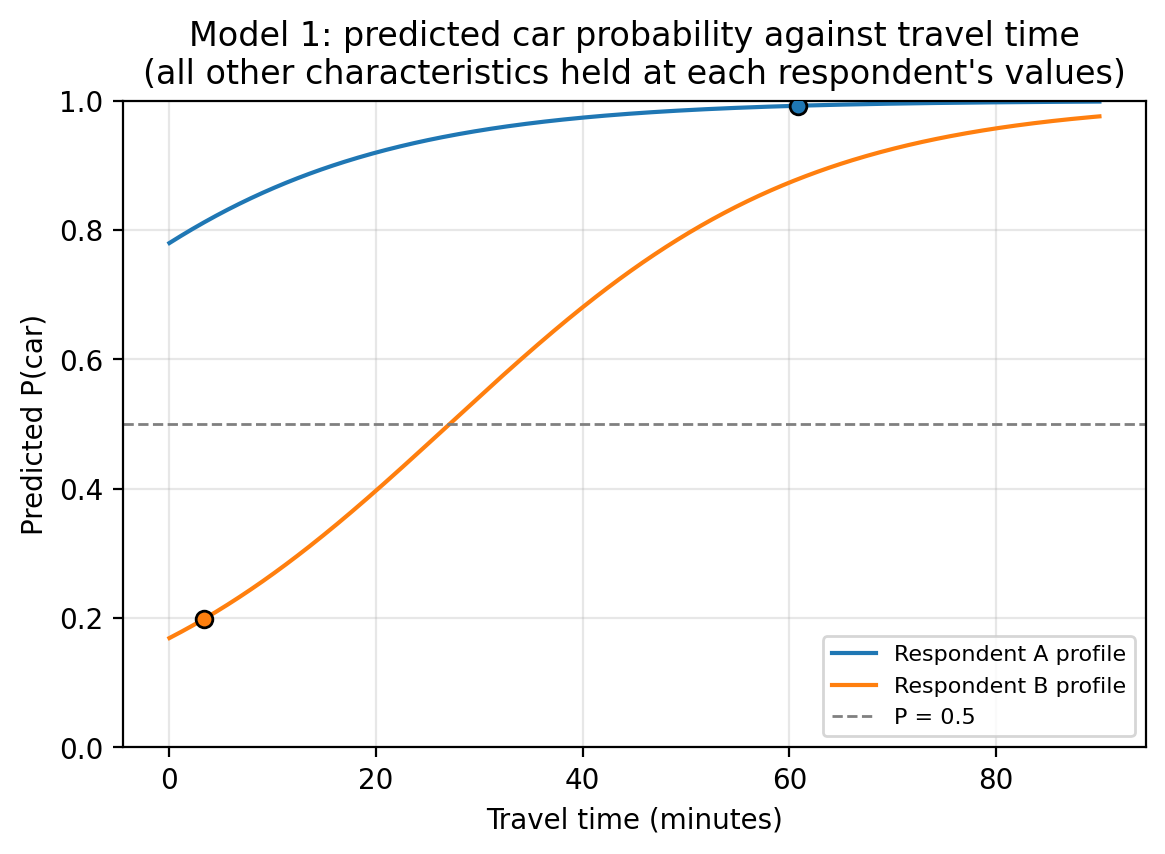
\includegraphics[width=0.68\textwidth]{figures/p1_2_probability_curves.png}
\caption{Predicted car probability as a function of travel time for each respondent's
profile, with all other characteristics held at their observed values. The markers show
the two respondents at their actual travel times.}
\label{fig:p12}
\end{figure}

\paragraph{Interpretation.} The gap between the two predictions is large, and every part
of it is traceable to the inputs.

Respondent A faces a 3650-second trip --- about 61 minutes --- is 60 years old, travels 24
times in the survey period, and lives in a two-person household owning two cars. Every one
of these characteristics pushes the linear predictor upward. Travel time alone contributes
$+3.57$ and vehicle ownership $+2.02$, which together account for most of the total. With
odds of roughly 126 to 1, the model treats A as an almost certain car user. This is
behaviourally sensible: an hour-long trip is simply not a realistic walking journey, and
the household has the vehicles to make driving possible.

Respondent B faces a 200-second trip --- roughly three minutes --- is 26, travels less
often, and, decisively, lives alone with \emph{no} vehicle. Since \code{HHVeh} carries the
largest coefficient in the model, having zero vehicles removes the single strongest driver
of car use, contributing nothing where A gained $+2.02$. The short trip also contributes
almost nothing ($+0.20$). The result is a low probability of driving, which again matches
intuition: a three-minute journey is an obvious walking trip for someone with no car.

Two points deserve comment rather than being passed over. First, the model still assigns
about a 20\% chance of driving to a car-free household on a three-minute trip, which is
higher than one might expect. This reflects the composition of the survey --- 78.8\% of the
sample travelled by car --- so the model's baseline propensity to predict car use is high,
and it also reflects the fact that the available regressors do not capture access to a
vehicle from outside the household through lifts, car-sharing or taxis. The prediction
should be read as the average behaviour of people with B's recorded characteristics, not
as a statement about one individual.

Second, Figure~\ref{fig:p12} makes clear why the coefficients are not marginal effects. B
sits on the steep part of the logistic curve, so an extra ten minutes of travel time moves
the predicted probability substantially. A is already saturated near 1 and barely responds
to the same change. The same $\hat\beta$ therefore produces very different changes in
probability depending on where a respondent sits, which is the essential non-linearity of
the logit model and a key difference from the linear regressions of Problem Set 1.

% ---------------------------------------------------------------------
\subsection{Principal components analysis of the independent variables (10 points)}
\label{sec:pca}

\paragraph{Method.} Principal components analysis rotates the predictors into uncorrelated
linear combinations ordered by the variance they capture. Writing $\mathbf{Z}$ for the
standardised data matrix, the components are the eigenvectors $\mathbf{v}_j$ of the
correlation matrix
\begin{equation}
\mathbf{R} = \tfrac{1}{n-1}\mathbf{Z}^{\top}\mathbf{Z},
\qquad
\mathbf{R}\mathbf{v}_j = \lambda_j \mathbf{v}_j,
\label{eq:pca}
\end{equation}
and the eigenvalue $\lambda_j$ is the variance carried by component $j$. Because
$\operatorname{tr}(\mathbf{R}) = K$, the eigenvalues sum to the number of variables, here
$K=5$.

Two decisions had to be made before running the analysis.

\begin{enumerate}[label=(\roman*),leftmargin=2em]
\item \emph{\code{travel\_mode} is excluded.} It is the dependent variable of the models in
Sections 1.1--1.2, and the question asks for a PCA of the independent variables. Including
it would mix an outcome into an unsupervised decomposition of the predictors.
\item \emph{The variables are standardised}, so Equation~\eqref{eq:pca} operates on the
correlation matrix rather than the covariance matrix. This is essential here because travel
time is measured in seconds and reaches 37{,}764, while household size runs from 1 to 13.
Running the PCA on the raw data confirms the danger: the first component then accounts for
99.97\% of the variance and is simply travel time, which is an artefact of the measurement
unit and tells us nothing about the structure of the data.

I standardise using the \emph{sample} standard deviation ($\mathrm{ddof} = 1$) rather than
\code{StandardScaler}, which divides by the population standard deviation
($\mathrm{ddof} = 0$). The distinction is small but not cosmetic: with $\mathrm{ddof} = 0$
the standardised variables have sample variance $n/(n-1) = 1.0002$, so the eigenvalues
would sum to $5.0010$ rather than to $K = 5$ exactly, contradicting the identity
$\operatorname{tr}(\mathbf{R}) = K$ stated above. Using $\mathrm{ddof} = 1$ makes the
sample covariance of $\mathbf{Z}$ exactly the correlation matrix. The explained-variance
proportions are identical either way.
\end{enumerate}

\paragraph{Data.} The file \code{mode\_choice\_pcasample.csv} contains 5000 rows and 6
columns with \textbf{no missing values}. There are 46 fully duplicated rows; since four of
the five predictors take small integer values, repeats are plausible genuine observations
rather than data errors, so they were retained. The five predictors entering the analysis
are \code{TrvlTime\_number} (seconds), \code{Age} (years),
\code{indiv\_trvl\_frequency} (count), \code{HHVeh} (vehicles) and \code{HHsize}
(persons). Travel time is severely right-skewed (skewness 11.01).

\begin{figure}[H]
\centering
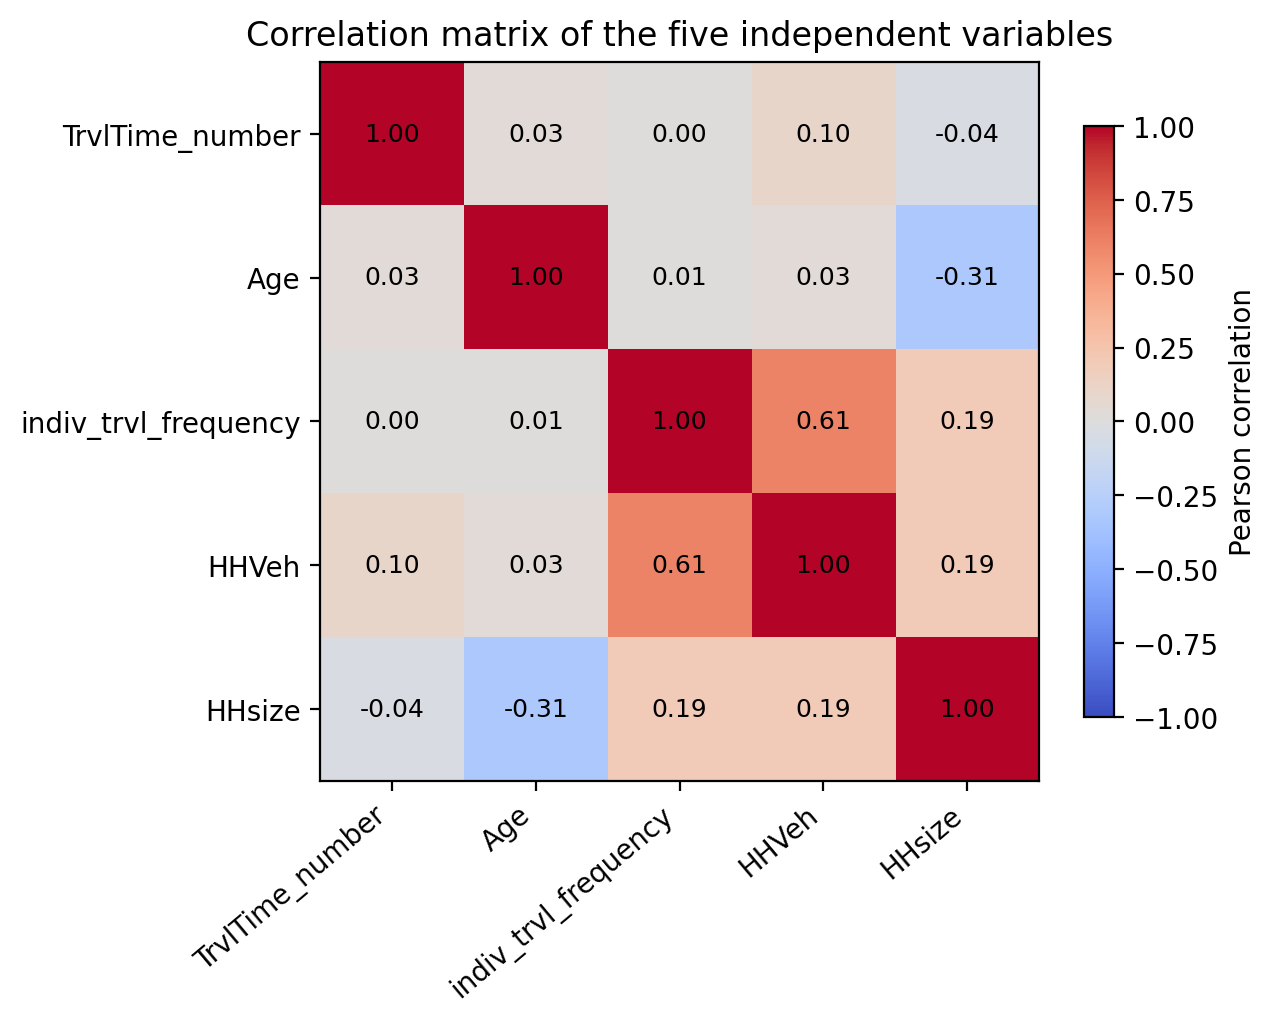
\includegraphics[width=0.60\textwidth]{figures/p1_3_correlation_matrix.png}
\caption{Correlation matrix of the five independent variables.}
\label{fig:corr}
\end{figure}

\paragraph{Results.} Table~\ref{tab:eigen} reports the eigenvalue spectrum and
Figure~\ref{fig:scree} shows it graphically.

\begin{table}[H]
\centering
\caption{Eigenvalues and variance explained (correlation matrix, $n=5000$, $K=5$).}
\label{tab:eigen}
\begin{tabular}{lrrr}
\toprule
Component & Eigenvalue $\lambda_j$ & Proportion of variance & Cumulative proportion \\
\midrule
PC1 & 1.7248 & 0.3450 & 0.3450 \\
PC2 & 1.2668 & 0.2534 & 0.5983 \\
PC3 & 0.9867 & 0.1973 & 0.7957 \\
PC4 & 0.6386 & 0.1277 & 0.9234 \\
PC5 & 0.3831 & 0.0766 & 1.0000 \\
\midrule
Sum & 5.0000 & 1.0000 & \\
\bottomrule
\end{tabular}
\end{table}

\begin{figure}[H]
\centering
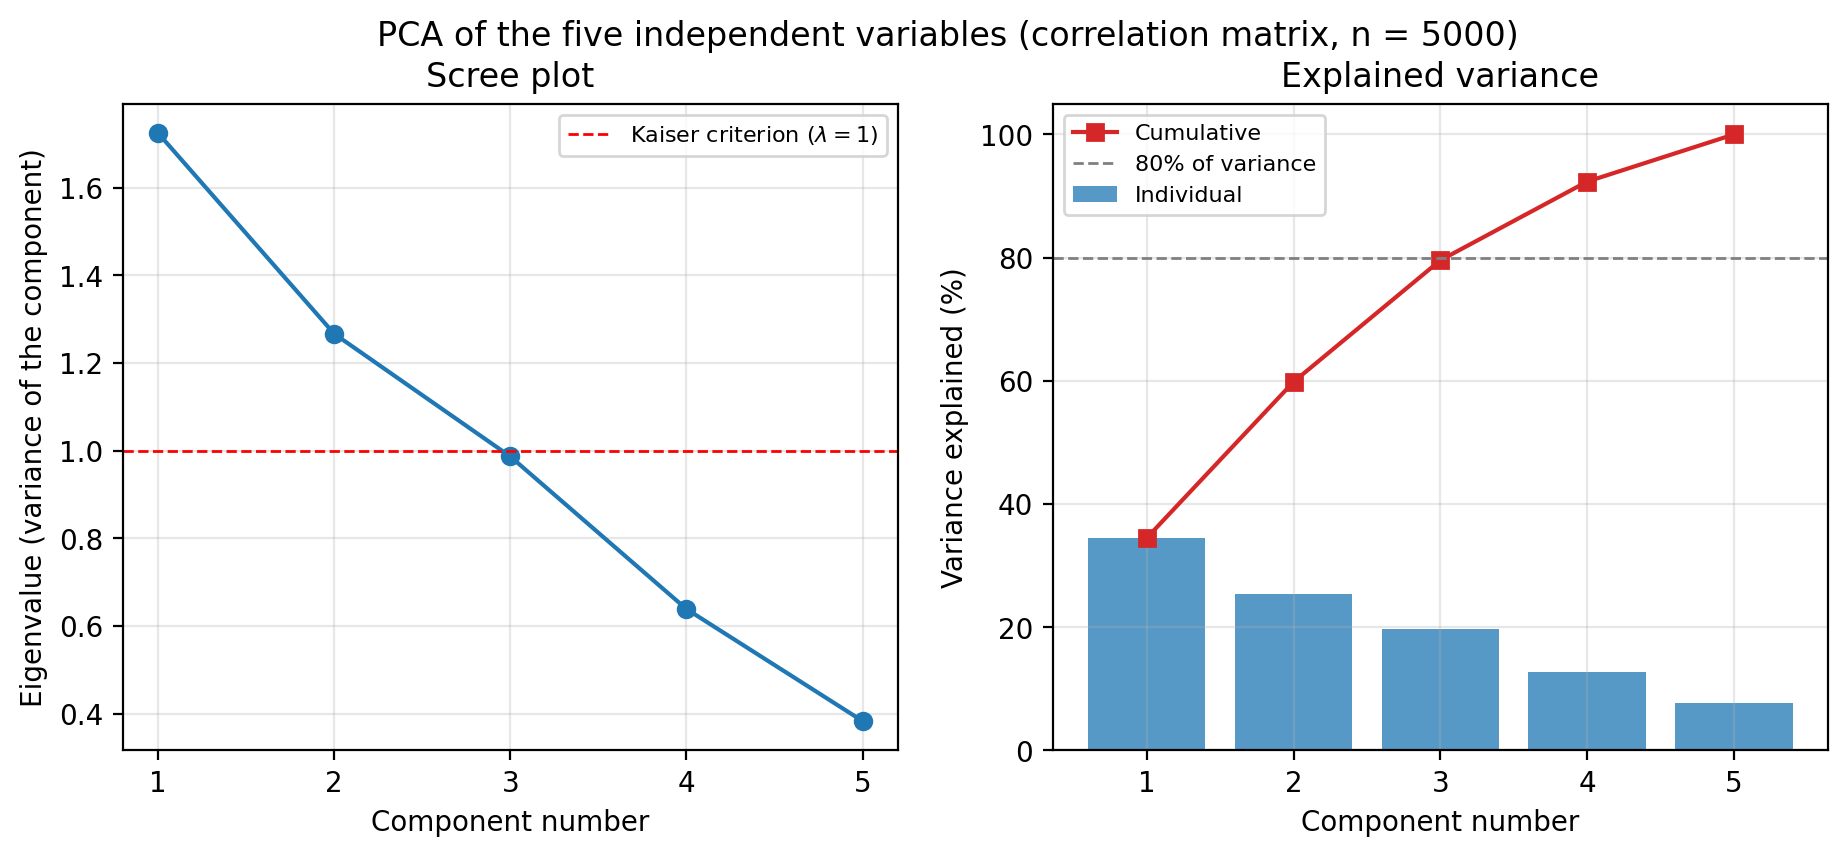
\includegraphics[width=0.92\textwidth]{figures/p1_3_scree_and_variance.png}
\caption{Scree plot with the Kaiser threshold (left) and individual and cumulative
variance explained (right).}
\label{fig:scree}
\end{figure}

\begin{table}[H]
\centering
\caption{Component loadings, that is the correlation between each original variable and
each component, computed as $v_{jk}\sqrt{\lambda_k}$. The final column gives the
communality retained by PC1--PC3.}
\label{tab:load}
\small
\begin{tabular}{lrrrrrr}
\toprule
Variable & PC1 & PC2 & PC3 & PC4 & PC5 & Communality (PC1--PC3) \\
\midrule
\code{TrvlTime\_number}      & $0.080$  & $0.289$  & $\mathbf{0.951}$ & $0.038$ & $-0.067$ & 0.994 \\
\code{Age}                   & $-0.170$ & $\mathbf{0.812}$ & $-0.221$ & $0.513$ & $-0.029$ & 0.736 \\
\code{indiv\_trvl\_frequency}& $\mathbf{0.843}$ & $0.232$  & $-0.162$ & $-0.167$& $-0.427$ & 0.790 \\
\code{HHVeh}                 & $\mathbf{0.846}$ & $0.284$  & $-0.022$ & $-0.087$& $0.441$  & 0.798 \\
\code{HHsize}                & $0.513$  & $\mathbf{-0.625}$& $0.082$  & $0.582$ & $-0.026$ & 0.661 \\
\bottomrule
\end{tabular}
\end{table}

\begin{figure}[H]
\centering
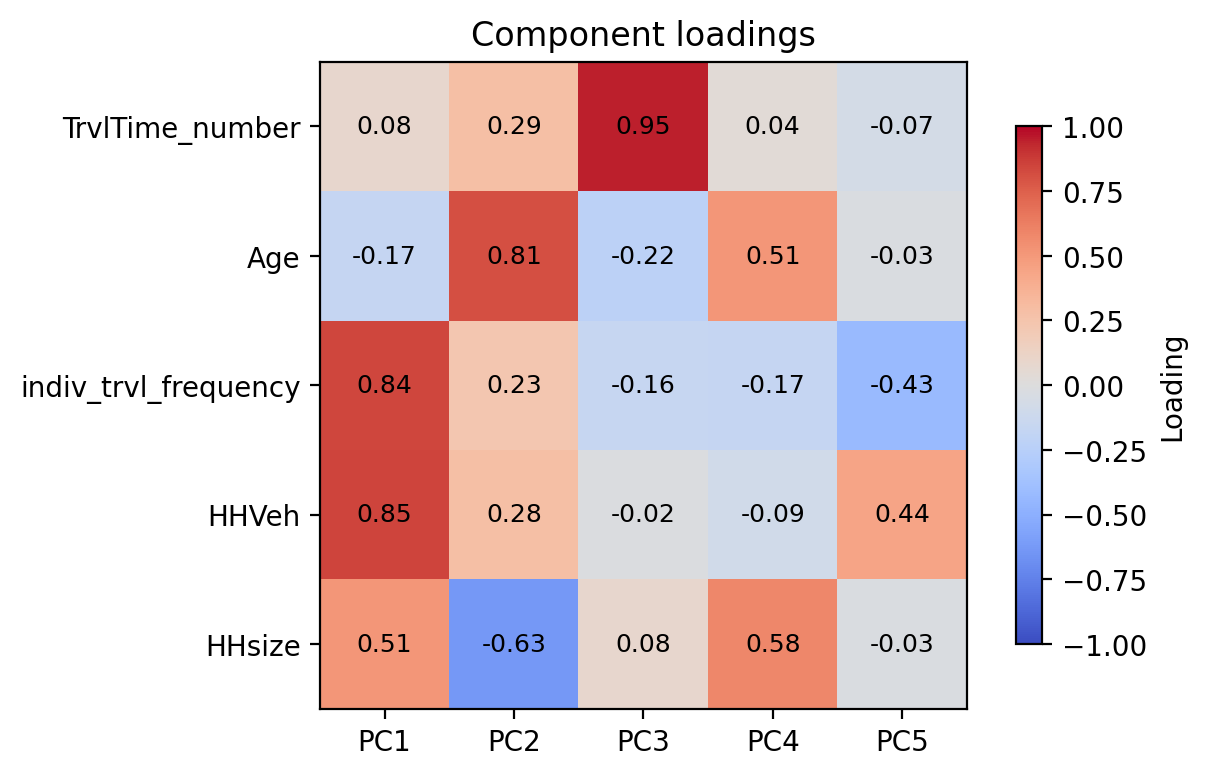
\includegraphics[width=0.60\textwidth]{figures/p1_3_loadings.png}
\hfill
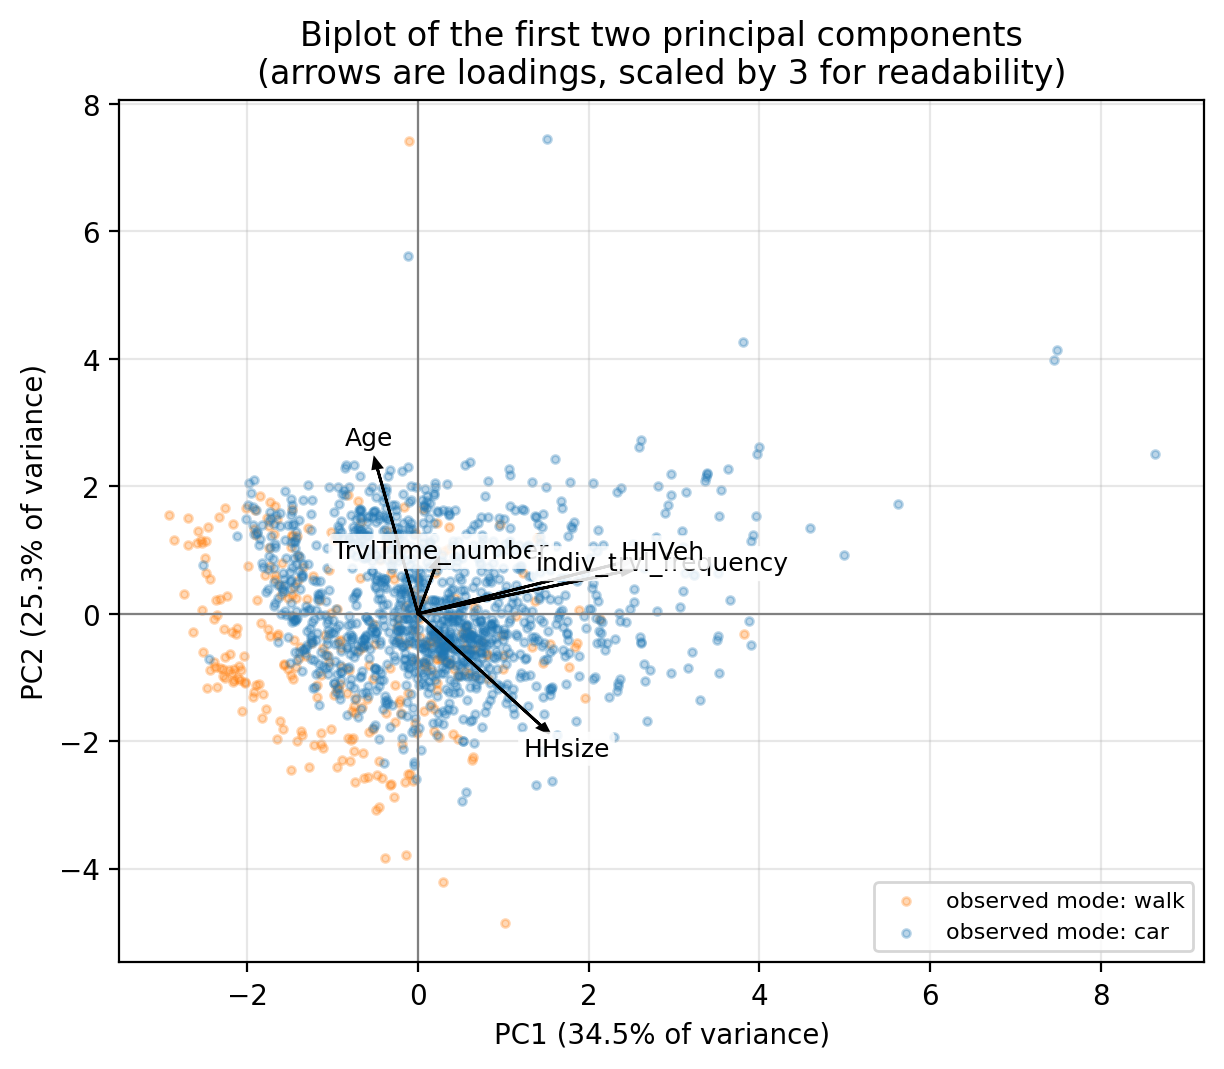
\includegraphics[width=0.60\textwidth]{figures/p1_3_biplot.png}
\caption{Component loadings (top) and biplot of the first two components (bottom). In the
biplot the points are observation scores, thinned to 1500 for readability and coloured by
the observed travel mode purely as a visual check --- \code{travel\_mode} played no part in
fitting the PCA.}
\label{fig:biplot}
\end{figure}

\paragraph{How many components to nominate.} The three standard rules do not agree, so
each is stated in turn.

\begin{itemize}[leftmargin=2em]
\item \emph{Kaiser criterion} ($\lambda_j > 1$): retain \textbf{two} components. However
$\lambda_3 = 0.9867$ misses the threshold by about 1\%, so this is a borderline exclusion
rather than a clear cut.
\item \emph{Cumulative variance}: PC1--PC2 retain 59.8\%, and adding PC3 brings the total
to 79.6\%. That is marginally short of the customary 80\% target; strictly, \textbf{four}
components would be needed to exceed it, which would leave almost no reduction at all.
\item \emph{Scree plot}: there is no sharp elbow. The eigenvalues decline gently from 1.73
to 0.38.
\end{itemize}

\textbf{I nominate three components}, retaining 79.6\% of the total variance. Since neither
mechanical rule selects three outright, the choice needs an argument. PC3 sits essentially
on the Kaiser boundary and takes the cumulative share to within half a percentage point of
the 80\% target, so on both criteria it is a marginal inclusion rather than a clear
exclusion. What settles it is substantive: PC3 is almost entirely travel time (loading
0.951), and travel time is the predictor most directly exposed to transport policy, since
service frequency, network design and congestion management all act on it, whereas age,
household size and vehicle ownership are socio-demographic characteristics an authority does
not control. Discarding the most policy-relevant dimension in the data in order to satisfy
thresholds it misses by a hundredth would be the wrong trade. Two components would
be defensible if the objective were strictly variance-driven compression, and I state that
alternative because the rules genuinely disagree.

\paragraph{Interpretation of the components.} PC1 (34.5\%) loads on
\code{indiv\_trvl\_frequency} ($0.843$), \code{HHVeh} ($0.846$) and \code{HHsize}
($0.513$). It is best read as \emph{household mobility resources and activity}: larger,
better-motorised households whose members travel more often. PC2 (25.3\%) contrasts
\code{Age} ($0.812$) against \code{HHsize} ($-0.625$), a \emph{life-stage} dimension that
separates older, smaller households from younger, larger ones. PC3 (19.7\%) is effectively
travel time on its own, consistent with travel time being almost uncorrelated with every
socio-demographic variable in the sample (all $|r| \le 0.10$ in Figure~\ref{fig:corr}).

\paragraph{Comment on the results.} The most useful finding is a negative one:
\textbf{PCA compresses this dataset rather little}. Five variables reduce to three at the
cost of 20.4\% of the variance, which is a modest saving. The reason is visible in
Figure~\ref{fig:corr}: only one pair of variables is appreciably correlated
($r = 0.609$ between \code{indiv\_trvl\_frequency} and \code{HHVeh}), while every other
pair sits below $0.32$ in absolute value. PCA can only exploit redundancy that exists, and
here there is little of it.

The communalities in Table~\ref{tab:load} show what three components actually preserve of
each variable. Travel time is almost fully retained ($0.994$), but \code{HHVeh} keeps
$0.798$, \code{indiv\_trvl\_frequency} $0.790$, \code{Age} $0.736$ and \code{HHsize} only
$0.661$ --- so a third of the variation in household size is lost even under the more
generous choice.

This contrasts instructively with the freeway data of Problem Set 1, where flow and
occupancy were near-duplicates with variance inflation factors above 90 and dimension
reduction was clearly warranted. Here the survey predictors carry largely independent
information, and a modeller would be better served by keeping the original variables, which
are directly interpretable in transport terms, than by substituting components that are
harder to explain to a practitioner. The one place where redundancy does exist is exactly
the correlation between \code{indiv\_trvl\_frequency} and \code{HHVeh}, which is consistent
with the coefficient sensitivity observed in Section 1.1 --- a useful indication that the
two parts of this problem are describing the same feature of the data.

\paragraph{Assumptions and limitations.} PCA is defined on second moments, so it is
sensitive to heavy tails. Travel time has skewness 11.01, which is a concern; a sensitivity
check log-transforming that variable leaves the spectrum essentially unchanged (cumulative
variance for three components moves from 0.7957 to 0.7976), so the conclusion is robust on
this point. Two further limitations should be kept in mind. \code{HHVeh} and \code{HHsize}
are discrete counts rather than continuous variables, so the correlation matrix only
approximates their association. And PCA is unsupervised: a component carrying little
variance may still matter for predicting mode choice, so components should never be
selected for a classification model on the basis of eigenvalues alone.

% =====================================================================
\section{Problem 2 (30 points)}

The dataset consists of the eight points of Table 2 in the problem sheet, four in each
class.

% ---------------------------------------------------------------------
\subsection{Plotting the data (5 points)}

\begin{figure}[H]
\centering
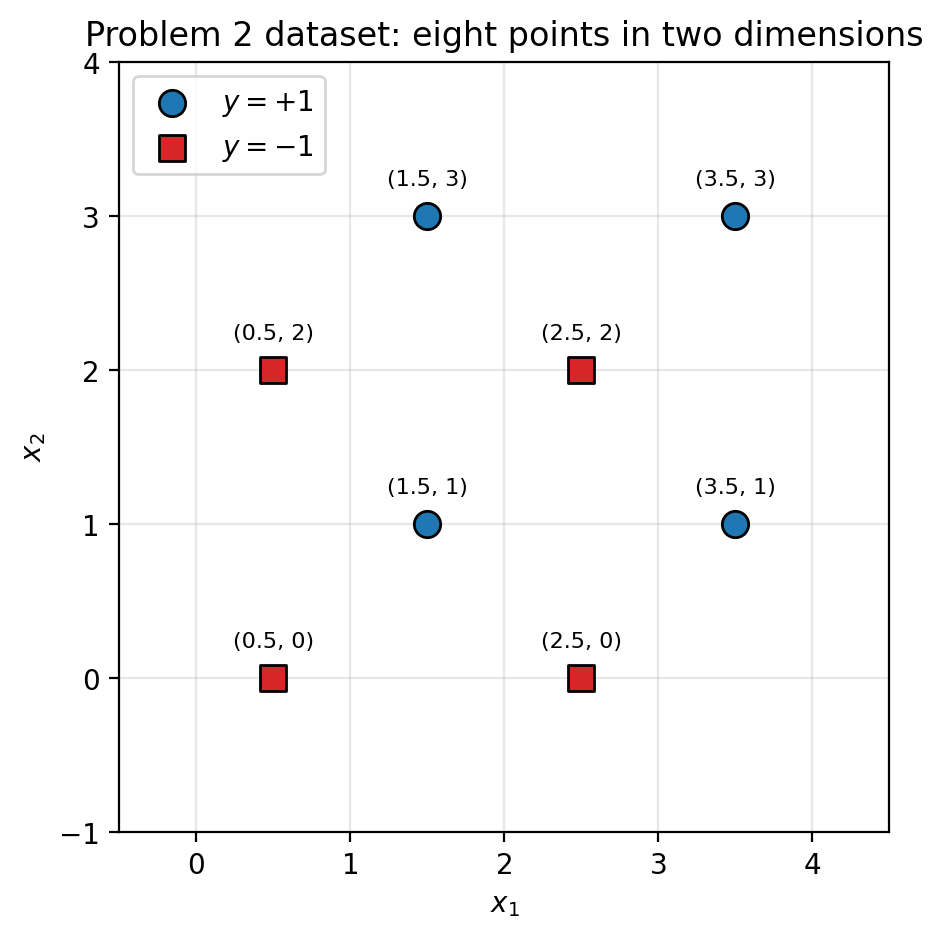
\includegraphics[width=0.55\textwidth]{figures/p2_1_data.png}
\caption{The eight data points, with the two classes shown by different markers: circles
for $y = +1$ and squares for $y = -1$.}
\label{fig:p21}
\end{figure}

The two classes interleave along both axes. Moving along $x_1$ the labels alternate
$-1, +1, -1, +1$ at $x_1 = 0.5, 1.5, 2.5, 3.5$, and moving along $x_2$ they alternate
$-1, +1, -1, +1$ at $x_2 = 0, 1, 2, 3$. No straight line can separate them, which is what
Sections 2.3--2.6 address.

% ---------------------------------------------------------------------
\subsection{Information gain rate of the rule $x_1 \ge 1$ (5 points)}

\paragraph{Method.} For a node $S$ with class proportions $p_k$ the entropy is
$H(S) = -\sum_k p_k \log_2 p_k$. Splitting $S$ into children $S_v$ gives
\begin{equation}
\mathrm{IG} = H(S) - \sum_v \frac{|S_v|}{|S|}H(S_v),
\qquad
\mathrm{SI} = -\sum_v \frac{|S_v|}{|S|}\log_2\frac{|S_v|}{|S|},
\qquad
\text{gain ratio} = \frac{\mathrm{IG}}{\mathrm{SI}} .
\label{eq:gr}
\end{equation}
The \emph{information gain rate}, also called the gain ratio, adjusts the raw gain by the
intrinsic information of the split. It mainly counters information gain's preference for
attributes with many branches, although it may itself favour highly unbalanced splits when
the split information is very small. Both quantities are reported below.

\paragraph{Calculation.} The parent node contains 4 positive and 4 negative points, so
\[
H(S) = -\tfrac12\log_2\tfrac12 - \tfrac12\log_2\tfrac12 = 1 \text{ bit.}
\]
The rule sends six points to the branch $x_1 \ge 1$, namely those at
$x_1 \in \{1.5, 2.5, 3.5\}$, of which four are positive and two negative, and two points to
the branch $x_1 < 1$, both negative:
\begin{align*}
H(x_1 \ge 1) &= -\tfrac46\log_2\tfrac46 - \tfrac26\log_2\tfrac26 = 0.918296, \\
H(x_1 < 1)   &= 0 \quad \text{(a pure leaf)}, \\
\sum_v \frac{|S_v|}{|S|}H(S_v) &= \tfrac68(0.918296) + \tfrac28(0) = 0.688722 .
\end{align*}
Substituting into Equation~\eqref{eq:gr},
\begin{align*}
\mathrm{IG} &= 1 - 0.688722 = \mathbf{0.311278 \text{ bits}}, \\
\mathrm{SI} &= -\tfrac68\log_2\tfrac68 - \tfrac28\log_2\tfrac28 = 0.811278 \text{ bits}, \\
\text{gain ratio} &= \frac{0.311278}{0.811278} = \mathbf{0.383689} .
\end{align*}

\paragraph{Interpretation.} The rule is informative but far from sufficient. It isolates
the two points at $x_1 = 0.5$ perfectly, producing a pure leaf, but the larger branch
remains impure because the points at $x_1 = 2.5$ are negative yet fall on the same side of
the threshold as all four positives. The rule classifies 6 of the 8 points correctly, an
accuracy of 75\%.

One detail is worth noting because it can look surprising: the gain ratio ($0.384$) is
\emph{larger} than the raw gain ($0.311$). For a \textbf{binary} split the split
information is $\mathrm{SI} = H\!\left(|S_L|/|S|\right)$, a function of a single
proportion. It attains its maximum of exactly one bit at an even $50/50$ partition and
\emph{decreases} as the partition becomes more uneven --- for example a $95/5$ split gives
$\mathrm{SI} = 0.286$. Hence $\mathrm{SI} \le 1$ always holds for a two-way split, and
dividing by it can only raise the score; here the $6/2$ partition gives
$\mathrm{SI} = 0.811$. Values of $\mathrm{SI}$ above one bit require more than two branches.

The gain ratio exists principally to counteract information gain's preference for
attributes with many possible values: it is what would penalise a rule splitting the eight
points into eight singleton branches, where $\mathrm{SI} = 3$ bits. A known side effect
runs in the opposite direction --- because a very uneven split has small $\mathrm{SI}$, the
gain ratio can itself favour highly unbalanced splits, which is usually managed by ranking
only those candidate splits whose raw information gain is at least average.

% ---------------------------------------------------------------------
\subsection{Soft margin linear SVM (5 points)}

\paragraph{Method.} The soft-margin ($C$-SVM) primal problem is
\begin{equation}
\min_{\mathbf{w},b,\boldsymbol{\xi}}\ \tfrac12\|\mathbf{w}\|^2 + C\sum_{i=1}^{n}\xi_i
\quad\text{subject to}\quad
y_i(\mathbf{w}^{\top}\mathbf{x}_i + b) \ge 1 - \xi_i,
\quad \xi_i \ge 0 .
\label{eq:svm}
\end{equation}
The slack variables $\xi_i$ allow points to violate the margin, and $C$ controls how
heavily violations are penalised relative to the margin width $2/\|\mathbf{w}\|$.

\paragraph{Why no linear model can succeed.} By the separating hyperplane theorem, two
finite point sets are linearly separable if and only if their convex hulls are disjoint.
Here the positive points form the rectangle $[1.5,\,3.5] \times [1,\,3]$ and the negative
points the rectangle $[0.5,\,2.5] \times [0,\,2]$. These intersect on
$[1.5,\,2.5] \times [1,\,2]$, so the hulls are \emph{not} disjoint and the data are
provably not linearly separable. The notebook verifies this constructively by exhibiting
the point $(2.0,\,1.5)$ of the intersection as a convex combination of the positive points,
with weights $(0.5625,\, 0.1875,\, 0.1875,\, 0.0625)$, and simultaneously of the negative
points, with weights $(0.0625,\, 0.1875,\, 0.1875,\, 0.5625)$. A single point cannot lie on
both sides of a hyperplane, so no linear boundary can classify all eight points correctly.

Consequently some $\xi_i$ must be positive at the optimum whatever $C$ is chosen, and zero
training error is unattainable. The model was fitted with $C = 1$ using scikit-learn's
\code{SVC} with a linear kernel, and a sweep over $C$ is reported to show that the
conclusion does not depend on that choice.

\paragraph{Results.} With $C = 1$ the fitted boundary is
\[
x_1 + x_2 - 3.5 = 0,
\]
with margin width $2/\|\mathbf{w}\| = 1.4142$ and six of the eight points acting as support
vectors. Training accuracy is $0.750$.

\begin{table}[H]
\centering
\caption{Behaviour of the soft-margin linear SVM as $C$ varies.}
\label{tab:csweep}
\begin{tabular}{rrrrrr}
\toprule
$C$ & $w_1$ & $w_2$ & $b$ & Margin $2/\|\mathbf{w}\|$ & Training accuracy \\
\midrule
0.1   & 0.3333 & 0.3333 & $-1.1667$ & 4.2426 & 0.750 \\
0.5   & 0.5000 & 0.5000 & $-1.7500$ & 2.8284 & 0.750 \\
1.0   & 1.0000 & 1.0000 & $-3.5000$ & 1.4142 & 0.750 \\
10.0  & 1.0000 & 1.0000 & $-3.5000$ & 1.4142 & 0.750 \\
100.0 & 1.0000 & 1.0000 & $-3.5000$ & 1.4142 & 0.750 \\
\bottomrule
\end{tabular}
\end{table}

\begin{figure}[H]
\centering
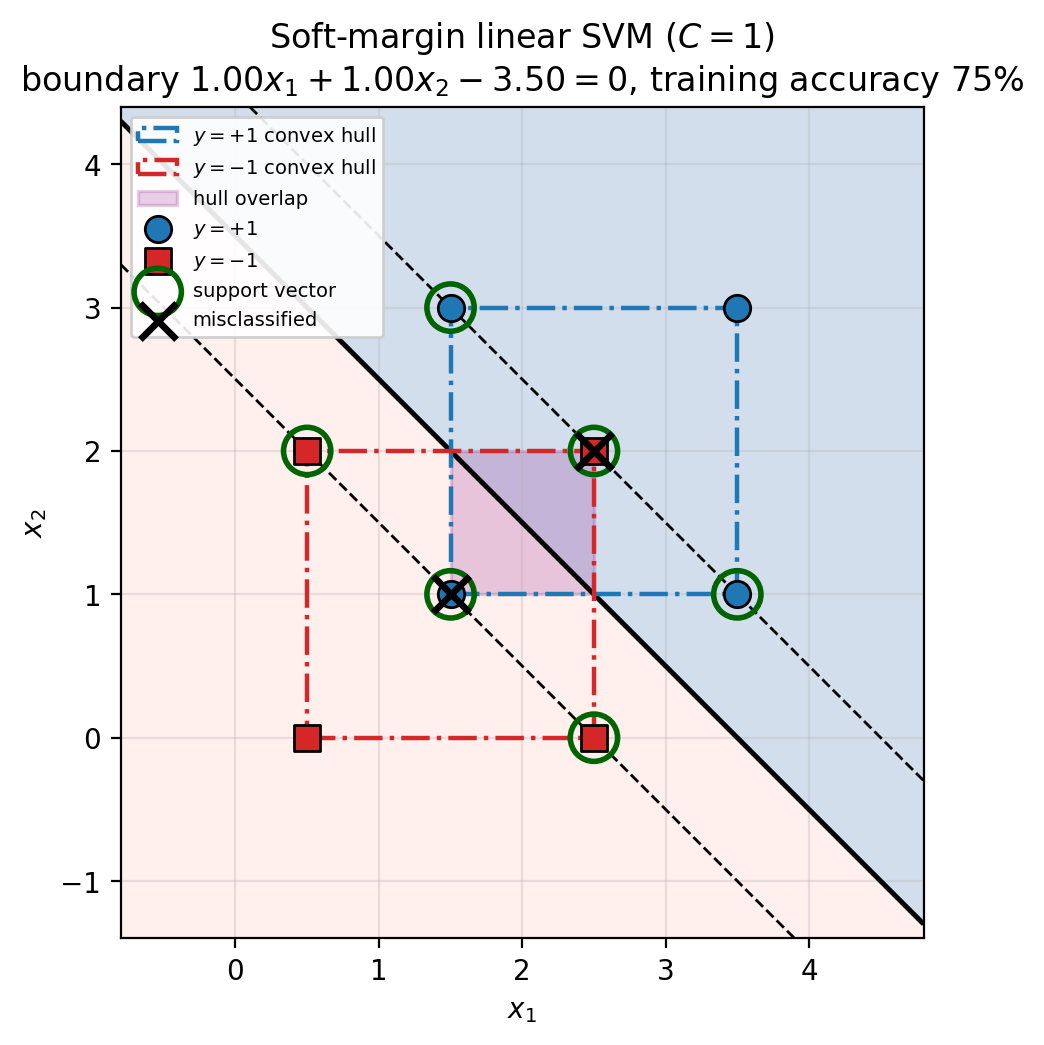
\includegraphics[width=0.62\textwidth]{figures/p2_3_linear_svm.png}
\caption{Soft-margin linear SVM with $C=1$. The solid line is the decision boundary, the
dashed lines the margins, green circles mark the support vectors and black crosses the two
misclassified points. The dash-dotted rectangles are the two class convex hulls; their
shaded intersection is why no linear boundary can separate the classes.}
\label{fig:p23}
\end{figure}

\paragraph{Interpretation.} The points $(1.5, 1.0)$ and $(2.5, 2.0)$ fall on the wrong side
of the boundary. Three of four correct in each class is the best any linear rule can
achieve here, and the convex-hull argument above explains why: the classes genuinely
overlap on $[1.5,\,2.5] \times [1,\,2]$, so any straight line must cut through points of
both classes. The failure is a property of the data, not of the optimiser.

The $C$ sweep in Table~\ref{tab:csweep} confirms this is structural. Every value from
$C = 0.1$ to $C = 100$ yields exactly the same 75\% training accuracy. Increasing $C$ only
shrinks the margin, from 4.243 at $C = 0.1$ to 1.414 from $C = 1$ upward, as the penalty on
slack grows and the model trades margin width for a tighter fit that it can never achieve.
This is precisely the situation that explicit feature maps and the kernel trick are designed
to address, and it motivates Sections 2.4--2.6.

% ---------------------------------------------------------------------
\subsection{An explicit mapping that makes the data separable (6 points)}

\paragraph{Reasoning.} Inspecting Figure~\ref{fig:p21}, the class labels are \emph{periodic}
in both coordinates with period 2. Positive points have $x_1 \in \{1.5, 3.5\}$ and
$x_2 \in \{1, 3\}$; negative points have $x_1 \in \{0.5, 2.5\}$ and $x_2 \in \{0, 2\}$.
Taking each coordinate modulo 2 removes the periodicity and collapses each class onto a
single point. Define $\varphi : \mathbb{R}^2 \to \mathbb{R}^2$ by
\begin{equation}
\varphi(x_1, x_2) = \bigl(x_1 \bmod 2,\ x_2 \bmod 2\bigr),
\label{eq:phi}
\end{equation}
using the mathematical modulus, whose result always lies in $[0,2)$, so that for example
$-0.5 \bmod 2 = 1.5$.

\paragraph{Results.} Under Equation~\eqref{eq:phi} all four positive points map to
$(1.5,\, 1.0)$ and all four negative points map to $(0.5,\, 0.0)$. The images are two
distinct points, so the mapped data are trivially separable. A hard-margin linear SVM
fitted in the mapped space returns
\[
z_1 + z_2 - 1.5 = 0
\]
with training accuracy $1.000$.

\begin{figure}[H]
\centering
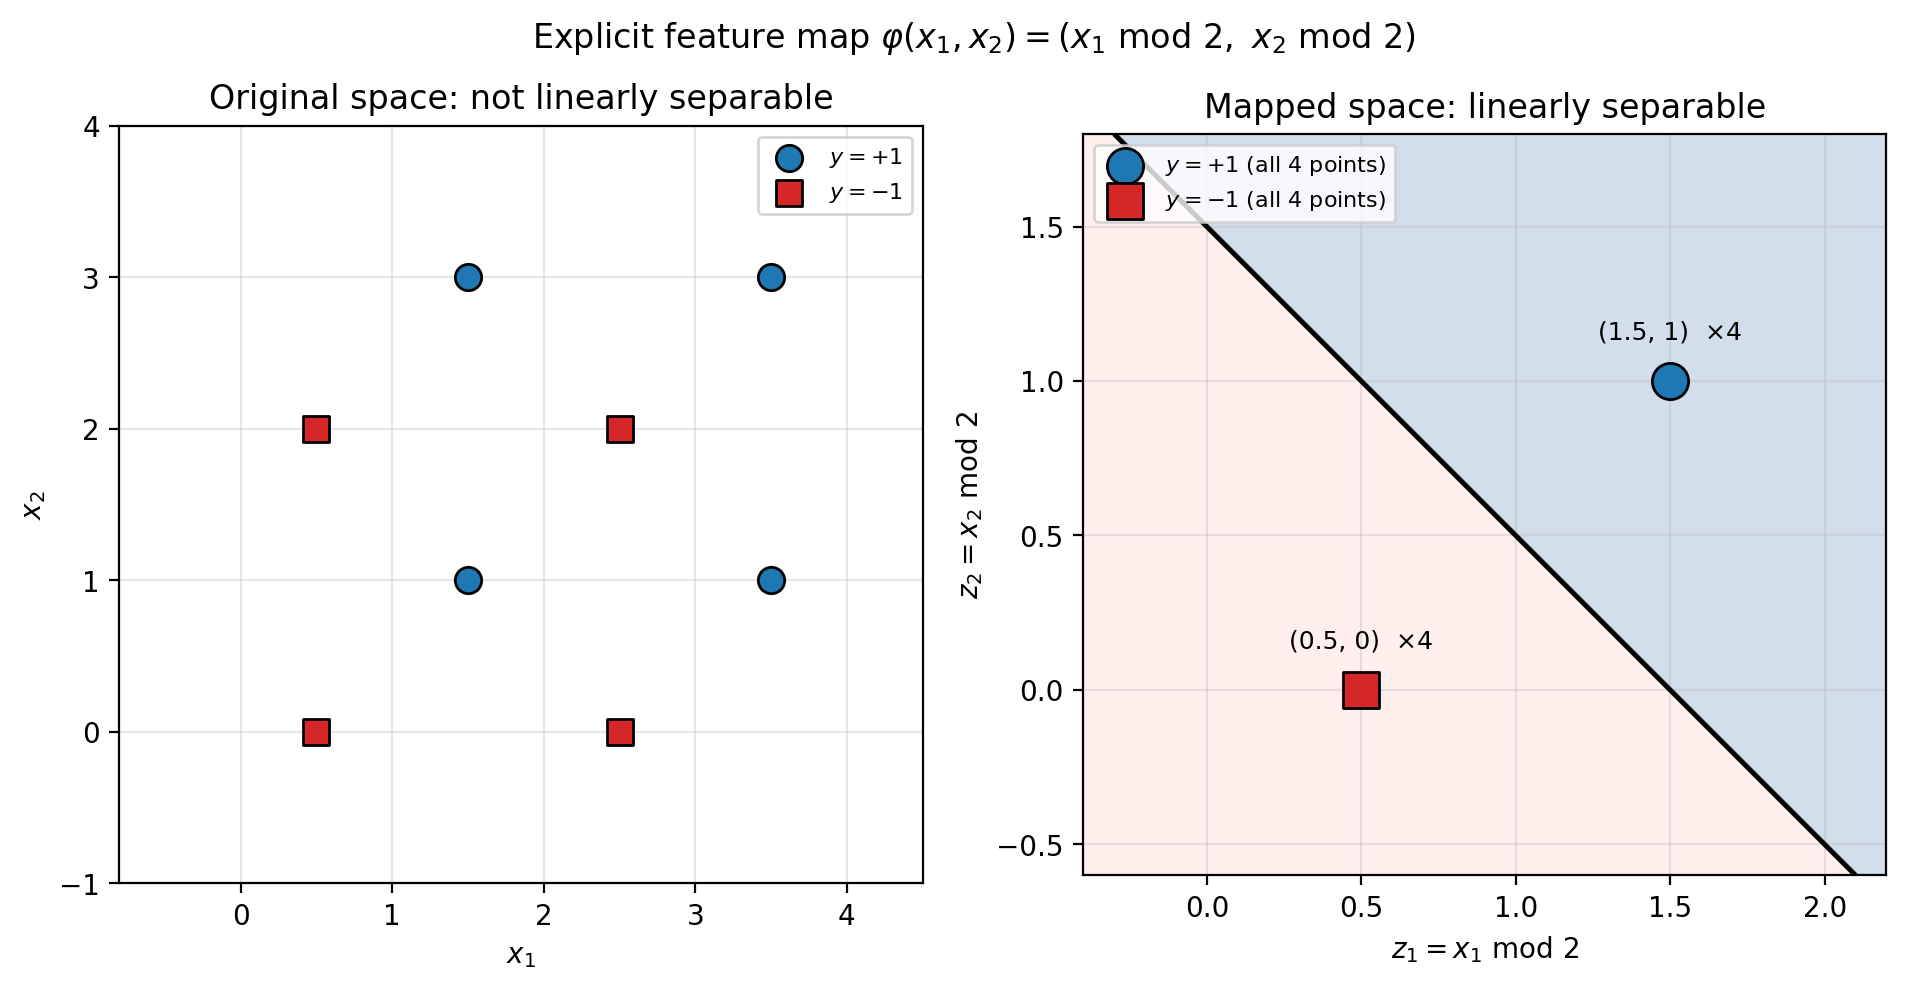
\includegraphics[width=0.92\textwidth]{figures/p2_4_feature_map.png}
\caption{The original space (left), where the classes interleave, and the mapped space
(right), where each class collapses to a single point and a line separates them. All four
points of each class coincide in the right-hand panel.}
\label{fig:p24}
\end{figure}

A smooth alternative with the same period-2 structure is
\begin{equation}
\tilde\varphi(x_1, x_2) = \bigl(\sin \pi x_1,\ \cos \pi x_2\bigr),
\label{eq:phitrig}
\end{equation}
which sends the positive points to $(-1,-1)$ and the negative points to $(+1,+1)$. It is
verified in Section 2.5 that both maps give identical predictions, so the answer does not
hinge on which is used.

\paragraph{Interpretation and limitation.} The map is deliberately lossy. It discards which
period a point falls in and retains only its position within the period. That is exactly the
right information to discard for this problem, because the label depends only on the
position within the period. The price is that $\varphi$ is not injective, so it would be the
wrong choice for any problem in which absolute position carries information.

% ---------------------------------------------------------------------
\subsection{Predictions for four new samples (4 points)}

Applying Equation~\eqref{eq:phi} to each new point and classifying with the rule
$z_1 + z_2 \gtrless 1.5$ obtained in Section 2.4 gives Table~\ref{tab:newpred}.

\begin{table}[H]
\centering
\caption{Predictions for the four new samples under the mapping of
Equation~\eqref{eq:phi}, with the smooth map of Equation~\eqref{eq:phitrig} as a check.}
\label{tab:newpred}
\begin{tabular}{rrrrrcc}
\toprule
$x_1$ & $x_2$ & $z_1 = x_1 \bmod 2$ & $z_2 = x_2 \bmod 2$ & $z_1 + z_2$ &
$\hat y$ & $\hat y$ (smooth map) \\
\midrule
$-0.5$ & $1.0$ & $1.5$ & $1.0$ & $2.5$ & $+1$ & $+1$ \\
$-0.5$ & $3.0$ & $1.5$ & $1.0$ & $2.5$ & $+1$ & $+1$ \\
$0.5$  & $4.0$ & $0.5$ & $0.0$ & $0.5$ & $-1$ & $-1$ \\
$2.5$  & $4.0$ & $0.5$ & $0.0$ & $0.5$ & $-1$ & $-1$ \\
\bottomrule
\end{tabular}
\end{table}

\begin{figure}[H]
\centering
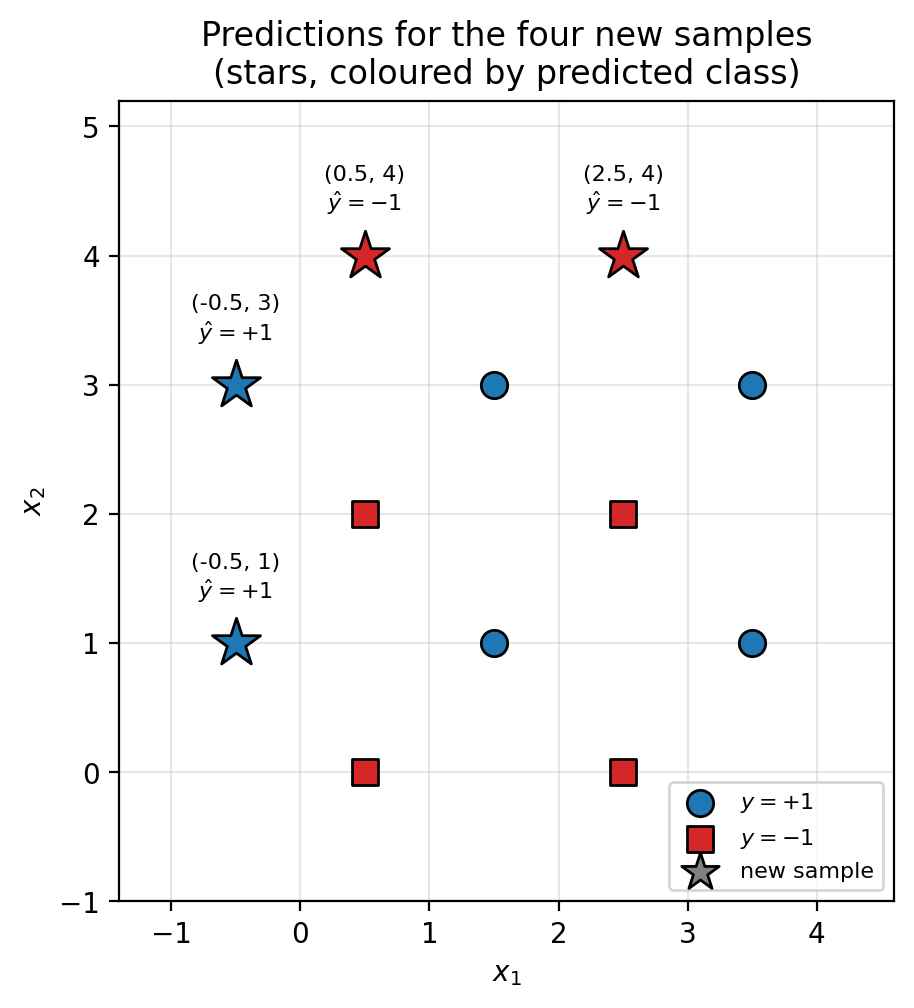
\includegraphics[width=0.55\textwidth]{figures/p2_5_new_predictions.png}
\caption{The four new samples shown as stars, coloured by their predicted class, together
with the original training points.}
\label{fig:p25}
\end{figure}

\paragraph{Interpretation and limitation.} The points $(-0.5, 1.0)$ and $(-0.5, 3.0)$ both
map onto the positive image and are predicted $\hat y = +1$; $(0.5, 4.0)$ and $(2.5, 4.0)$
both map onto the negative image and are predicted $\hat y = -1$. The two feature maps agree
on every point.

These are extrapolations rather than interpolations: $x_1 = -0.5$ lies below the observed
range of $x_1$ and $x_2 = 4.0$ above the observed range of $x_2$. The predictions therefore
rest on the assumption that the period-2 structure continues beyond the training data, which
eight points cannot verify. The predictions should be treated as conditional on that
assumption.

% ---------------------------------------------------------------------
\subsection{The kernel trick and the kernel matrix (5 points)}

\paragraph{Method.} The kernel trick replaces the inner product
$\varphi(\mathbf{x}_i)^{\top}\varphi(\mathbf{x}_j)$ in the dual form of the SVM by a kernel
function $K(\mathbf{x}_i, \mathbf{x}_j)$ evaluated directly on the original inputs, so the
feature map never has to be formed explicitly. For $n$ training points the Gram (kernel)
matrix is $\mathbf{K} \in \mathbb{R}^{n\times n}$ with
$K_{ij} = K(\mathbf{x}_i, \mathbf{x}_j)$. I use the Gaussian (RBF) kernel
\begin{equation}
K(\mathbf{x}, \mathbf{z}) = \exp\left(-\gamma\|\mathbf{x}-\mathbf{z}\|^2\right),
\qquad \gamma = 0.5,
\label{eq:rbf}
\end{equation}
and alongside it, for comparison, the kernel induced by the smooth feature map
$\tilde\varphi$ of Equation~\eqref{eq:phitrig}:
\begin{equation}
K_{\tilde\varphi}(\mathbf{x},\mathbf{z})
= \tilde\varphi(\mathbf{x})^{\top}\tilde\varphi(\mathbf{z})
= \sin(\pi x_1)\sin(\pi z_1) + \cos(\pi x_2)\cos(\pi z_2).
\label{eq:kphi}
\end{equation}
I use $\tilde\varphi$ here rather than the modulo map because it sends both classes to
images of equal norm, $(-1,-1)$ and $(+1,+1)$, so its inner products are directly
comparable across pairs. The modulo map sends the classes to $(1.5, 1)$ and $(0.5, 0)$,
whose norms differ by a factor of three; an un-centred inner product between vectors of
unequal length confounds similarity of direction with magnitude, so that Gram matrix cannot
be read directly as a similarity structure even though the map itself classifies perfectly.
The points are ordered with the four positives first so that any class block structure is
visible.

\begin{figure}[H]
\centering
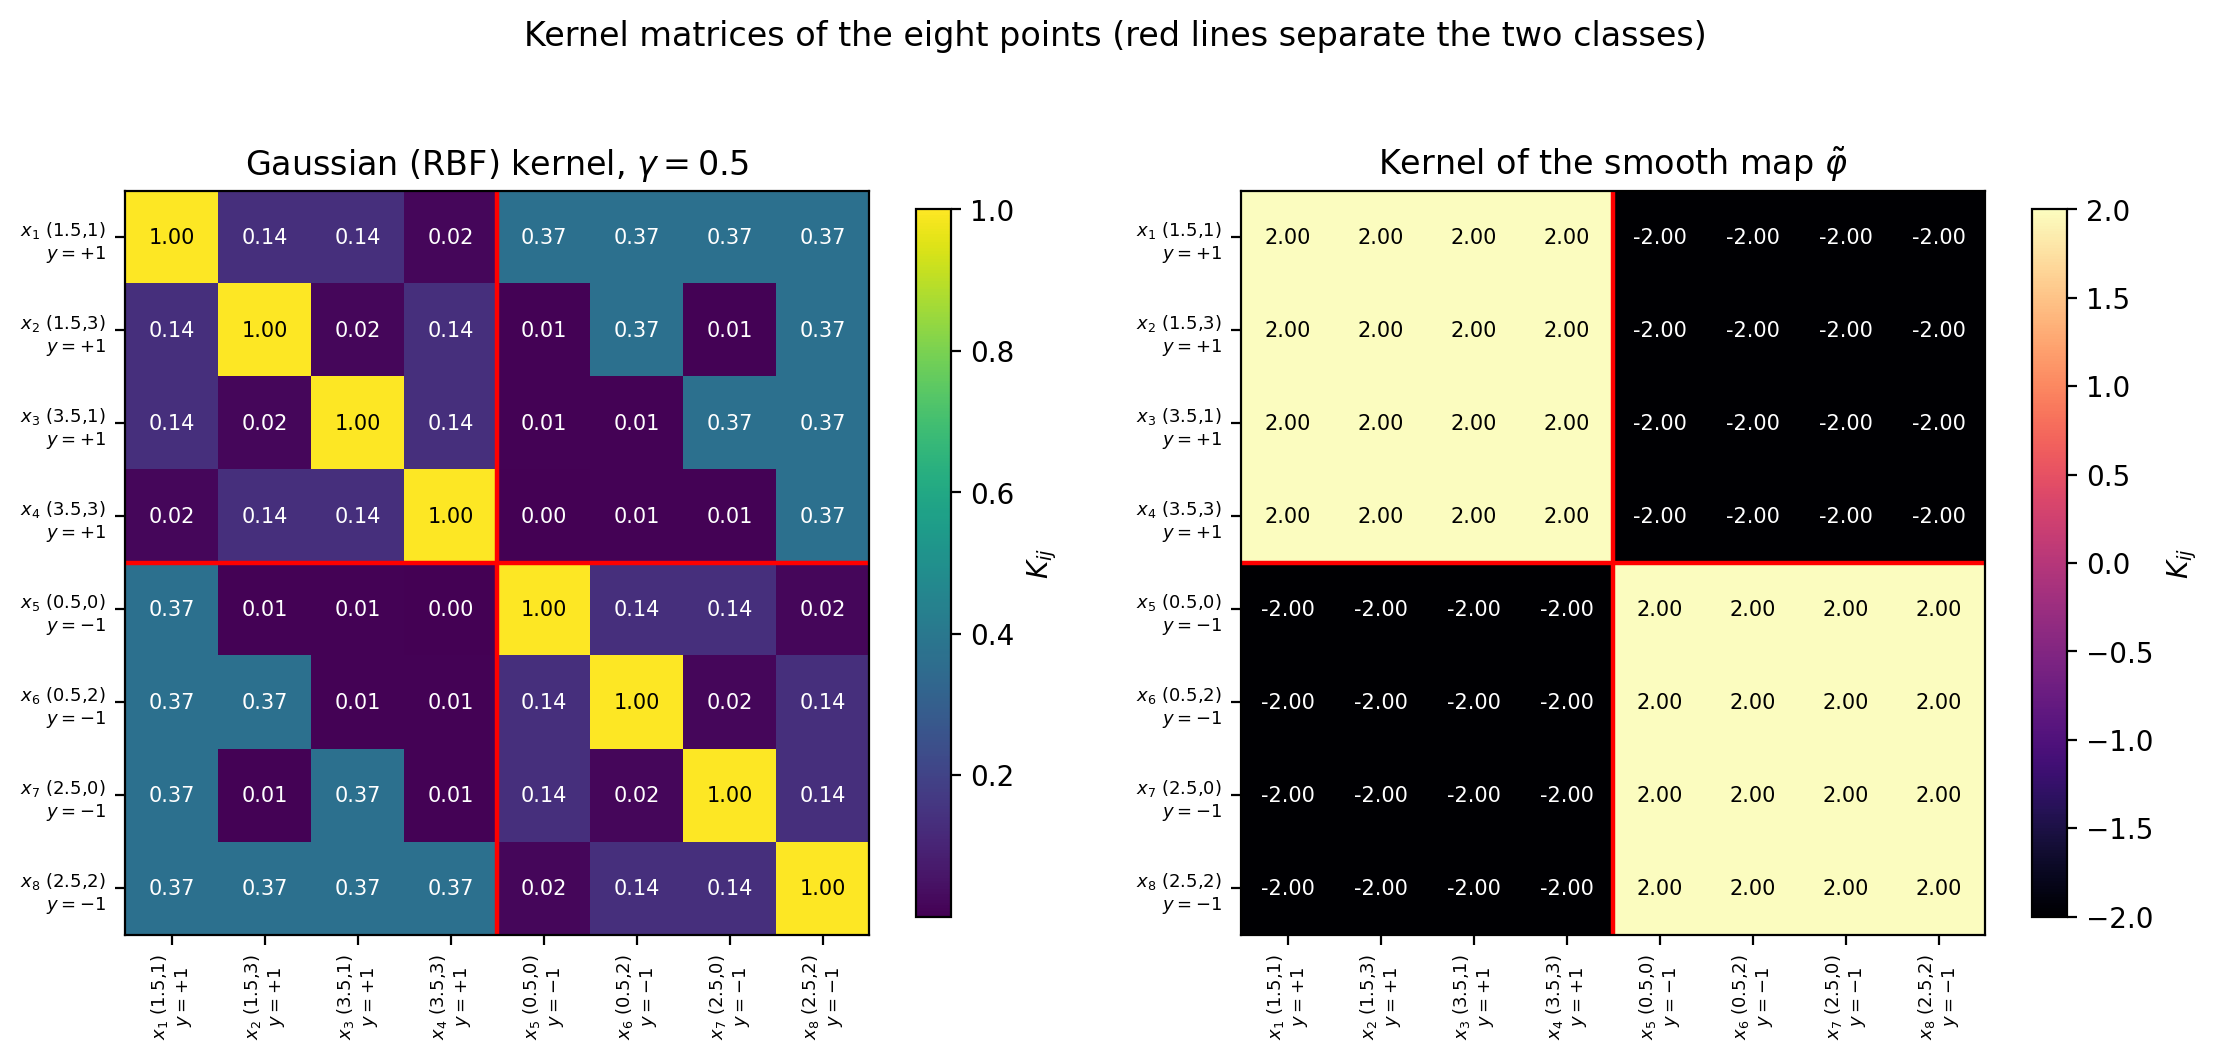
\includegraphics[width=\textwidth]{figures/p2_6_kernel_matrices.png}
\caption{Kernel matrices of the eight points. Left: the Gaussian kernel of
Equation~\eqref{eq:rbf}. Right: the kernel induced by the smooth map $\tilde\varphi$,
Equation~\eqref{eq:kphi}. Red lines separate the two classes; rows and columns 1--4 are the
positive class.}
\label{fig:p26}
\end{figure}

\paragraph{Interpretation.} The RBF matrix has ones on the diagonal, since
$K(\mathbf{x},\mathbf{x}) = 1$, and decays with squared distance. All eight of its
eigenvalues are positive (the smallest is $0.2802$), confirming that it is a valid positive
semi-definite kernel, as Mercer's condition requires.

The revealing feature is that the class blocks marked by the red lines are \emph{not}
uniformly bright. Several within-class entries are close to zero --- for example
$K_{14} = 0.018$, between $(1.5, 3.0)$ and $(3.5, 1.0)$, which share a label but sit far
apart --- while several cross-class entries are comparatively large, with every entry in the
first column of the lower-left block equal to $0.368$. This is exactly the interleaving that
defeated the linear SVM in Section 2.3, now expressed in terms of similarity: with
$\gamma = 0.5$ the Gaussian kernel measures plain geometric proximity, and geometric
proximity does not track the class label in this dataset. An RBF SVM would still fit the
training set, because a sufficiently large $\gamma$ can fit almost anything, but it would be
memorising the points rather than exploiting their structure.

The kernel of Equation~\eqref{eq:kphi} shows what a well-matched kernel looks like: an
exact $4 \times 4$ block structure with $K_{ij} = +2$ for every pair in the same class and
$K_{ij} = -2$ for every pair in different classes. Because both class images have the same
norm, $\sqrt{2}$, these values are directly comparable, and every point is strictly more similar
to all four members of its own class than to any member of the other --- precisely the
condition that fails for the Gaussian kernel. That is why a linear classifier separates the
mapped data perfectly.

The contrast makes the practical lesson of the kernel trick concrete: the choice of kernel
encodes an assumption about which points should count as similar, and a kernel matched to
the structure of the problem does far more work than a generic one. It is worth adding a
note of caution about reading Gram matrices in general. An un-centred inner product mixes
similarity of direction with magnitude, so a block of large entries does not by itself
demonstrate within-class similarity unless the feature images are comparably scaled, as
they are here. Where they are not, a normalised kernel such as
$K(\mathbf{x},\mathbf{z}) / \sqrt{K(\mathbf{x},\mathbf{x}) K(\mathbf{z},\mathbf{z})}$ is
the appropriate quantity to inspect.

% =====================================================================
\section{Problem 3 (35 points)}

Throughout this problem $Y = 1$ denotes a severe delay and $Y = 0$ a non-severe delay, in
the context of a public transport control centre predicting whether an operational incident
will escalate.

% ---------------------------------------------------------------------
\subsection{Decision-tree splitting criteria (12 points)}

The node holds 12 historical incidents, 7 severe and 5 non-severe. With
$H(S) = -\sum_k p_k\log_2 p_k$ and $G(S) = 1 - \sum_k p_k^2$, a binary split into children
$S_L$ and $S_R$ is scored by
\begin{equation}
\mathrm{IG} = H(S) - \frac{|S_L|}{|S|}H(S_L) - \frac{|S_R|}{|S|}H(S_R),
\qquad
\Delta G = G(S) - \frac{|S_L|}{|S|}G(S_L) - \frac{|S_R|}{|S|}G(S_R).
\label{eq:split}
\end{equation}

\subsubsection*{3.1.1 Entropy and Gini impurity of the parent node (3 points)}

With $p_1 = 7/12 = 0.583333$ and $p_0 = 5/12 = 0.416667$,
\begin{align*}
H(S) &= -\tfrac{7}{12}\log_2\tfrac{7}{12} - \tfrac{5}{12}\log_2\tfrac{5}{12}
      = \mathbf{0.979869 \text{ bits}}, \\
G(S) &= 1 - \left(\tfrac{7}{12}\right)^2 - \left(\tfrac{5}{12}\right)^2
      = 1 - 0.513889 = \mathbf{0.486111}.
\end{align*}
The node is close to maximally impure, as expected from a nearly even 7:5 class split.

\subsubsection*{3.1.2 Weighted child entropy and information gain (3 points)}

\emph{Split A} (\code{current\_delay\_min} $\ge 10$): left child 5 severe and 1 non-severe
($n_L = 6$), right child 2 severe and 4 non-severe ($n_R = 6$).
\begin{align*}
H(S_L) &= -\tfrac56\log_2\tfrac56 - \tfrac16\log_2\tfrac16 = 0.650022, \qquad
H(S_R)  = -\tfrac26\log_2\tfrac26 - \tfrac46\log_2\tfrac46 = 0.918296, \\
\text{weighted } H &= \tfrac{6}{12}(0.650022) + \tfrac{6}{12}(0.918296) = 0.784159, \\
\mathrm{IG}_A &= 0.979869 - 0.784159 = \mathbf{0.195710 \text{ bits}}.
\end{align*}

\emph{Split B} (\code{major\_incident} = yes): left child 5 severe and 0 non-severe
($n_L = 5$), right child 2 severe and 5 non-severe ($n_R = 7$).
\begin{align*}
H(S_L) &= 0 \quad\text{(pure)}, \qquad
H(S_R)  = -\tfrac27\log_2\tfrac27 - \tfrac57\log_2\tfrac57 = 0.863121, \\
\text{weighted } H &= \tfrac{5}{12}(0) + \tfrac{7}{12}(0.863121) = 0.503487, \\
\mathrm{IG}_B &= 0.979869 - 0.503487 = \mathbf{0.476382 \text{ bits}}.
\end{align*}

\subsubsection*{3.1.3 Weighted child Gini impurity and Gini reduction (3 points)}

\emph{Split A}:
\begin{align*}
G(S_L) &= 1 - \left(\tfrac56\right)^2 - \left(\tfrac16\right)^2 = 0.277778, \qquad
G(S_R)  = 1 - \left(\tfrac26\right)^2 - \left(\tfrac46\right)^2 = 0.444444, \\
\text{weighted } G &= \tfrac12(0.277778) + \tfrac12(0.444444) = 0.361111, \\
\Delta G_A &= 0.486111 - 0.361111 = \mathbf{0.125000}.
\end{align*}

\emph{Split B}:
\begin{align*}
G(S_L) &= 0 \quad\text{(pure)}, \qquad
G(S_R)  = 1 - \left(\tfrac27\right)^2 - \left(\tfrac57\right)^2 = 0.408163, \\
\text{weighted } G &= \tfrac{5}{12}(0) + \tfrac{7}{12}(0.408163) = 0.238095, \qquad
\Delta G_B = 0.486111 - 0.238095 = \mathbf{0.248016}.
\end{align*}

\begin{table}[H]
\centering
\caption{Summary of the two candidate splits at the root node.}
\label{tab:splits}
\small
\begin{tabular}{lrrrr}
\toprule
Split & Weighted $H$ & Information gain & Weighted $G$ & Gini reduction \\
\midrule
Parent & --- & --- & --- & --- \\
A: \code{current\_delay\_min} $\ge 10$ & 0.784159 & 0.195710 & 0.361111 & 0.125000 \\
B: \code{major\_incident} = yes        & 0.503487 & \textbf{0.476382} & 0.238095 & \textbf{0.248016} \\
\bottomrule
\end{tabular}
\end{table}

\begin{figure}[H]
\centering
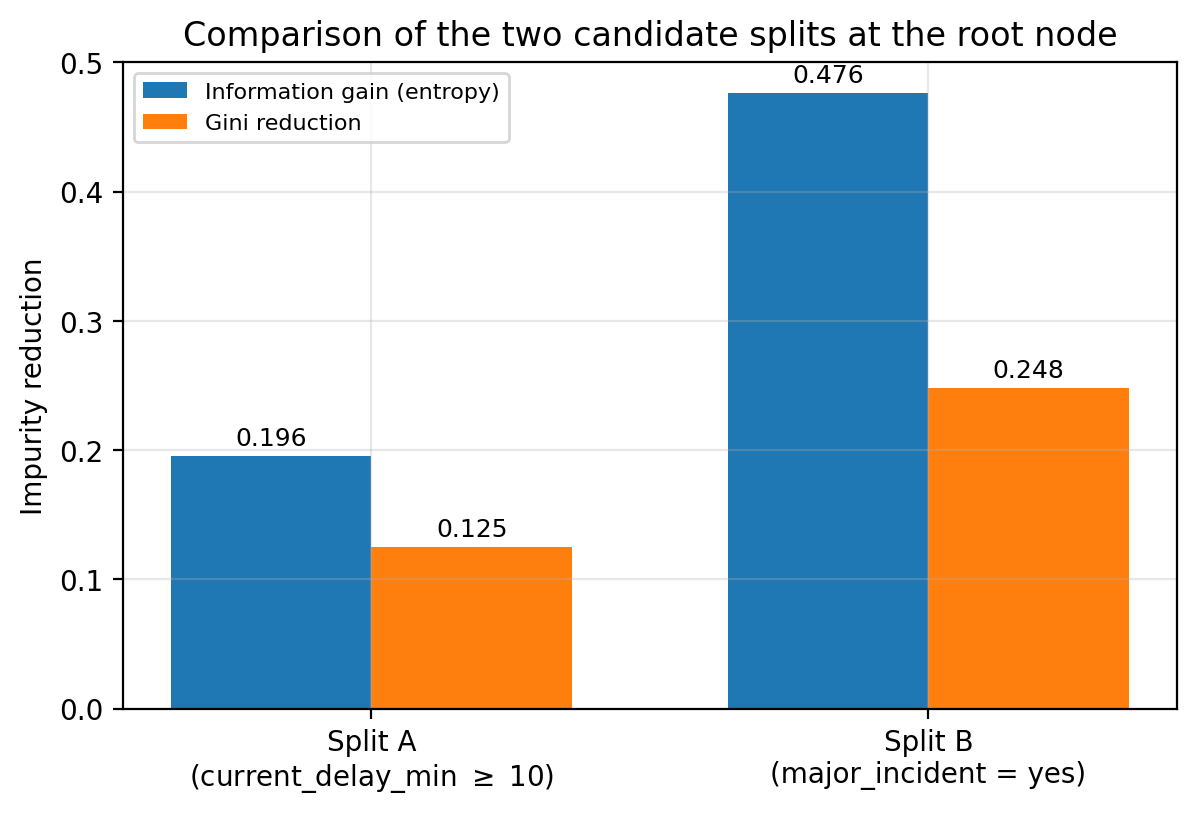
\includegraphics[width=0.60\textwidth]{figures/p3_1_split_comparison.png}
\caption{Impurity reduction achieved by each candidate split under both criteria.}
\label{fig:p31}
\end{figure}

\subsubsection*{3.1.4 Which split should be selected first? (3 points)}

\textbf{Split B should be selected first}, because it gives both the larger information gain
($0.476382$ against $0.195710$ bits) and the larger Gini reduction ($0.248016$ against
$0.125000$), so the two criteria agree. In control-centre terms, \code{major\_incident} = yes
isolates a completely pure group of severe delays, which makes it an immediately actionable
first split that can trigger escalation without waiting to see how the delay develops.

% ---------------------------------------------------------------------
\subsection{Bootstrap sampling and out-of-bag observations (9 points)}

\subsubsection*{3.2.1 Probability that observation $i$ is or is not selected (3 points)}

A bootstrap sample draws $n$ observations with replacement, each draw uniform over the $n$
original observations and independent of the others. A single draw selects observation $i$
with probability $1/n$, so it fails to select $i$ with probability $1 - 1/n$. Because the
$n$ draws are independent, the probabilities multiply:
\begin{equation}
P(i \notin \text{sample}) = \left(1 - \frac{1}{n}\right)^{n},
\qquad
P(i \in \text{sample}) = 1 - \left(1 - \frac{1}{n}\right)^{n} .
\label{eq:boot}
\end{equation}

\subsubsection*{3.2.2 Limiting values as $n \to \infty$ (2 points)}

Writing the first expression as an exponential,
\[
\left(1 - \frac{1}{n}\right)^{n} = \exp\left[n\ln\left(1 - \frac1n\right)\right],
\qquad
n\ln\left(1-\frac1n\right) = n\left(-\frac1n - \frac{1}{2n^2} - \cdots\right) \to -1,
\]
so
\[
\lim_{n\to\infty} P(i \notin \text{sample}) = e^{-1} = \mathbf{0.367879},
\qquad
\lim_{n\to\infty} P(i \in \text{sample}) = 1 - e^{-1} = \mathbf{0.632121}.
\]

\textbf{In words:} however large the dataset, a bootstrap sample contains only about 63\% of
the distinct observations and leaves roughly 37\% out-of-bag. Convergence is fast --- the
value is already $0.366032$ at $n = 100$, as Figure~\ref{fig:p32} shows. This is what makes
the trees in a bagged ensemble differ from one another, and it supplies a validation set at
no cost: each tree can be scored on the roughly one third of the data it never saw, which is
the basis of the out-of-bag error estimate used by random forests.

\begin{figure}[H]
\centering
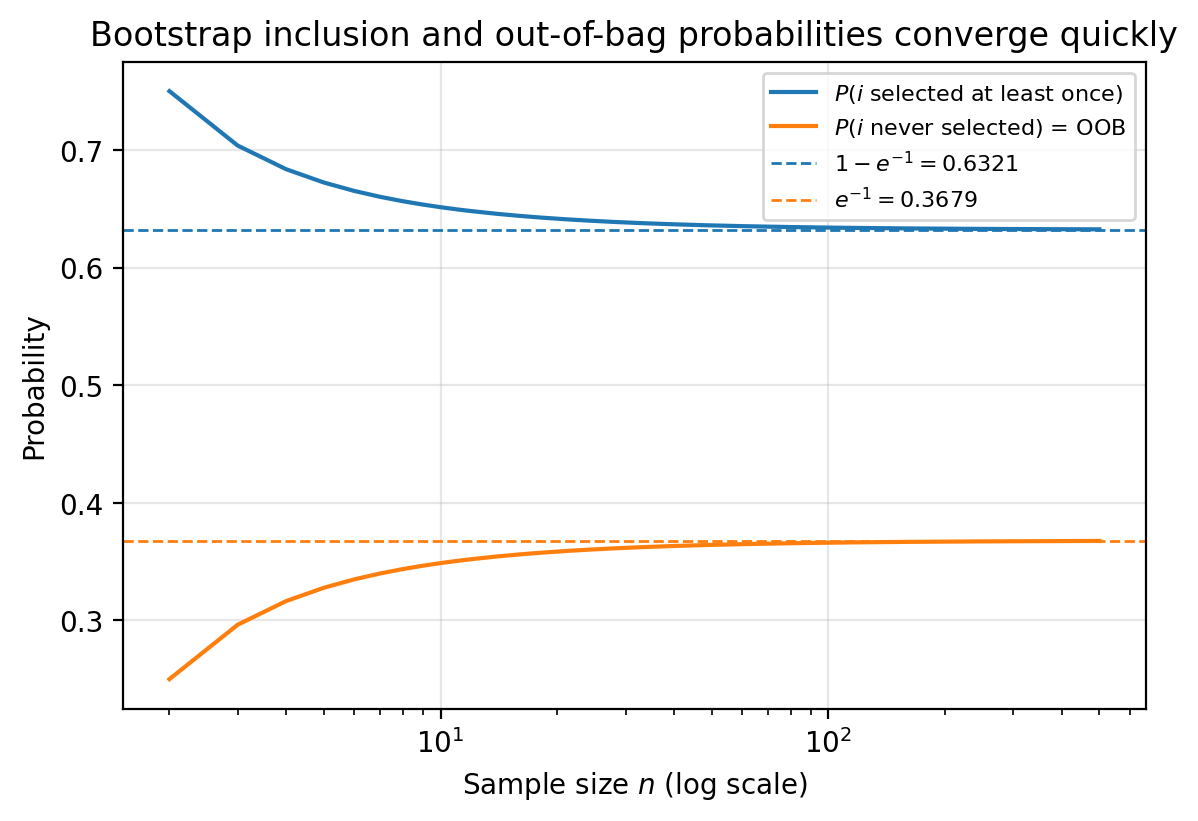
\includegraphics[width=0.60\textwidth]{figures/p3_2_bootstrap_probabilities.png}
\caption{Inclusion and out-of-bag probabilities as a function of sample size, converging
rapidly to $1 - e^{-1}$ and $e^{-1}$.}
\label{fig:p32}
\end{figure}

\subsubsection*{3.2.3 Expected unique and out-of-bag observations for $n = 5000$ (2 points)}

Substituting $n = 5000$ into Equation~\eqref{eq:boot} gives
$P(i \notin \text{sample}) = 0.367843$. By linearity of expectation, summing the indicator
over all $n$ observations,
\begin{align*}
\mathbb{E}[\text{unique observations}] &= n\left[1 - \left(1-\tfrac1n\right)^n\right]
  = 5000 \times 0.632157 = \mathbf{3160.79} \quad (63.22\%), \\
\mathbb{E}[\text{out-of-bag observations}] &= n\left(1-\tfrac1n\right)^n
  = 5000 \times 0.367843 = \mathbf{1839.21} \quad (36.78\%).
\end{align*}
A simulation of 2000 bootstrap samples in the notebook gives 3159.55 unique and 1840.45
out-of-bag on average, confirming the algebra.

\subsubsection*{3.2.4 Counting bootstrap samples from five incidents (2 points)}

For $\{A, B, C, D, E\}$ with a sample of size 5:
\begin{itemize}[leftmargin=2em]
\item \textbf{Ordered samples.} Each of the 5 draws independently has 5 possible outcomes,
so the number of ordered samples is $5^5 = \mathbf{3125}$.
\item \textbf{Unordered datasets.} If only the multiplicities of $A,\dots,E$ matter, the
count is the number of multisets of size 5 drawn from 5 types, given by the
stars-and-bars formula
\[
\binom{n + k - 1}{k} = \binom{5 + 5 - 1}{5} = \binom{9}{5} = \mathbf{126}.
\]
\end{itemize}
The large gap between 3125 and 126 shows that most of the ordered samples are permutations
of one another; since a decision tree does not care about the order in which its training
rows are presented, 126 is the number of genuinely distinct training sets available.

% ---------------------------------------------------------------------
\subsection{Ensemble voting and boosting intuition (4 points)}

\subsubsection*{3.3.1 Majority vote of five independent classifiers (2 points)}

With $M = 5$ independent classifiers each correct with probability $p = 0.65$, the number
correct is $X \sim \mathrm{Bin}(5, 0.65)$ and the majority vote is right when $X \ge 3$:
\begin{align*}
P(X \ge 3) &= \sum_{k=3}^{5}\binom{5}{k}(0.65)^k(0.35)^{5-k} \\
&= \underbrace{10(0.65)^3(0.35)^2}_{0.336416}
 + \underbrace{5(0.65)^4(0.35)^1}_{0.312386}
 + \underbrace{(0.65)^5}_{0.116029}
 = \mathbf{0.764831}.
\end{align*}
Combining five weak classifiers lifts accuracy from 65\% to 76.5\%, a gain of 11.5
percentage points.

\begin{figure}[H]
\centering
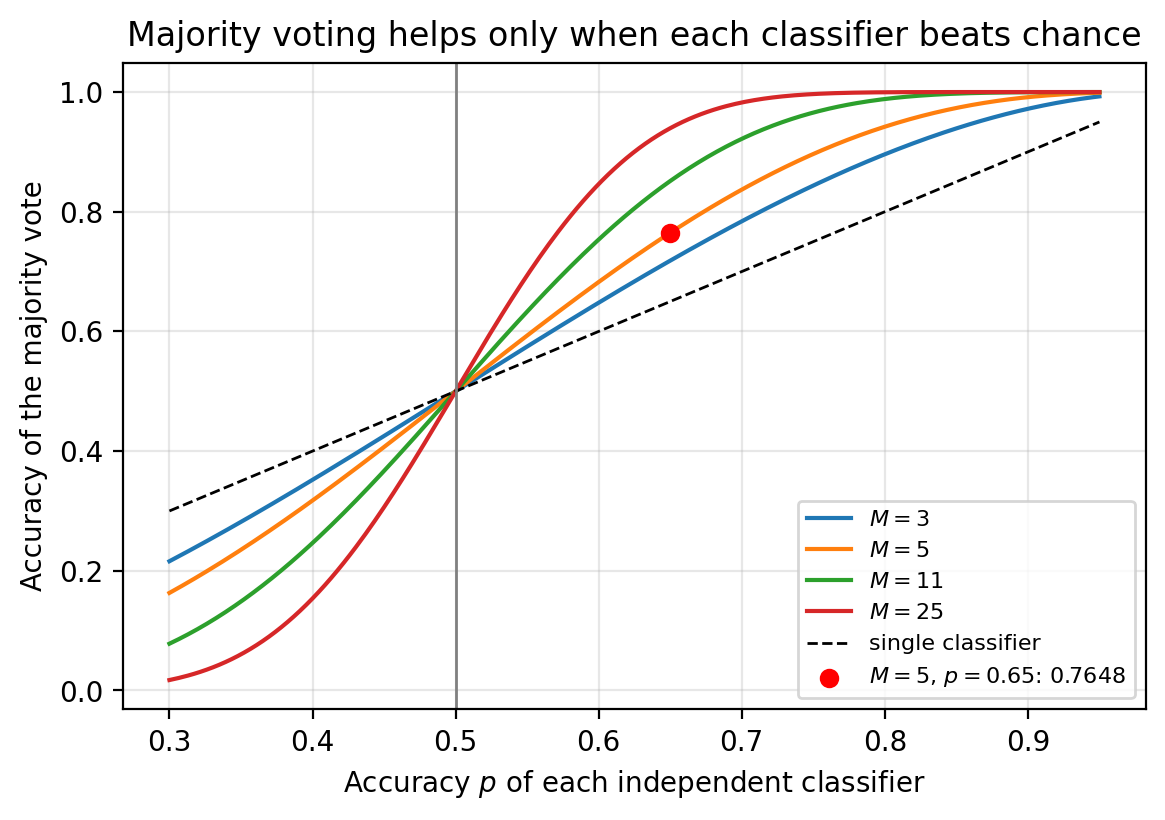
\includegraphics[width=0.58\textwidth]{figures/p3_3_majority_vote.png}
\caption{Accuracy of a majority vote as a function of the individual accuracy $p$, for
different ensemble sizes $M$.}
\label{fig:p33}
\end{figure}

Figure~\ref{fig:p33} shows the condition under which this works: the vote improves on the
individual classifier only when $p > 0.5$, and below that adding classifiers makes matters
worse. The calculation also assumes independence, which real ensemble members never fully
satisfy. A random forest only approximates independence through bootstrap sampling and
random feature subsets, so the realised gain in practice is smaller than this idealised
figure.

\subsubsection*{3.3.2 One gradient boosting update (2 points)}

With $y = [5, 9, 14, 18]$ and $\hat y^{(0)} = [8, 8, 8, 8]$, the residuals are
\[
r_i = y_i - \hat y^{(0)}_i = [-3,\ 1,\ 6,\ 10].
\]
Applying the update $\hat y^{(1)} = \hat y^{(0)} + \eta\, h_1(x)$ with $\eta = 0.2$ and
$h_1(x) = [-2, 1, 5, 5]$ gives Table~\ref{tab:boost}.

\begin{table}[H]
\centering
\caption{One gradient boosting update with learning rate $\eta = 0.2$.}
\label{tab:boost}
\begin{tabular}{crrrrrr}
\toprule
$i$ & $y_i$ & $\hat y^{(0)}_i$ & $r_i$ & $h_1(x_i)$ & $\eta\,h_1(x_i)$ & $\hat y^{(1)}_i$ \\
\midrule
1 & 5  & 8 & $-3$ & $-2$ & $-0.4$ & $\mathbf{7.6}$ \\
2 & 9  & 8 & $1$  & $1$  & $0.2$  & $\mathbf{8.2}$ \\
3 & 14 & 8 & $6$  & $5$  & $1.0$  & $\mathbf{9.0}$ \\
4 & 18 & 8 & $10$ & $5$  & $1.0$  & $\mathbf{9.0}$ \\
\bottomrule
\end{tabular}
\end{table}

So $\hat y^{(1)} = [7.6,\ 8.2,\ 9.0,\ 9.0]$.

Every prediction moves in the direction of its residual but only a fifth of the way, which
is the purpose of shrinkage: the sum of squared errors falls from 146.0 to 113.4 in one
step rather than jumping to a possibly over-fitted solution. The two largest residuals, 6
and 10, remain substantially unresolved after this round, so many further iterations would
be needed. This is the standard trade-off in boosting --- a small learning rate requires
more trees but generalises better than a large one.

% ---------------------------------------------------------------------
\subsection{Coding exercise: severe-delay prediction (10 points)}

\paragraph{Data and protocol.} The dataset was generated exactly as specified in the problem
sheet, using \code{np.random.default\_rng(42)} and $n = 1200$. Six operational features
describe each incident, and \code{severe\_delay} is a thresholded noisy score built from
main effects and interactions, so a good model must be able to represent interactions such
as \code{peak\_hour} \textsc{and} \code{rain}. There are no missing values. As required, a
stratified train--test split with 70\% training and 30\% test data was used with
\code{random\_state=42}, giving 840 training and 360 test incidents. Stratification
preserved the class proportions (severe share $0.2345$ in training and $0.2333$ in test).
The test set was used only for final evaluation. Every choice made during the analysis ---
the cross-validated model comparison in Section 3.4.3 and the threshold selection in
Section 3.4.5 --- was carried out on the training partition alone.

\subsubsection*{3.4.1 Class balance (1 point)}

Of the 1200 incidents, \textbf{919 (76.58\%) are non-severe and 281 (23.42\%) are severe},
an imbalance of about $3.27 : 1$.

\begin{figure}[H]
\centering
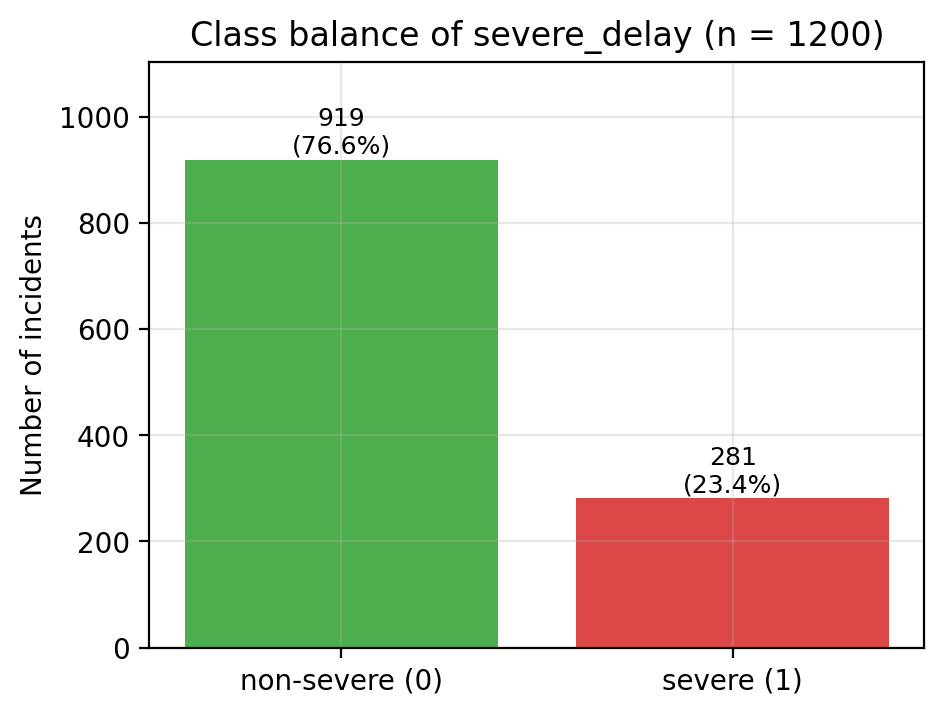
\includegraphics[width=0.42\textwidth]{figures/p3_4_class_balance.png}
\caption{Class balance of \code{severe\_delay}.}
\label{fig:p341}
\end{figure}

\paragraph{Why class balance matters in transportation applications.} There are two
connected reasons. First, imbalance makes accuracy misleading as a headline metric. A model
that predicts ``non-severe'' for every incident would score 76.6\% accuracy while providing
no operational value at all, so accuracy must always be read alongside recall, F1 and
ROC-AUC. This is confirmed empirically below, where the majority-class baseline achieves
0.7667 accuracy with an F1-score of exactly zero.

Second, and more importantly, the rare class is the one that matters. Severe delays are what
trigger replacement buses, staff callouts and passenger information --- they are the entire
reason the control centre wants a model. Training algorithms that minimise overall error
will, if left alone, sacrifice performance on the minority class to gain on the majority,
which is exactly the wrong trade for this application. The imbalance here is moderate, so
the models were trained on the data as generated, as the problem sheet specifies, rather
than reweighted; but the choice of metrics and the threshold discussion in Section 3.4.5
both take it into account.

\subsubsection*{3.4.2 Decision tree with \code{max\_depth=3} (1 point)}

\paragraph{First split.} The root split is on
\[
\code{current\_delay\_min} \le 7.4684 ,
\]
sending 628 training incidents to the left child (Gini $0.2433$, severe share $0.1417$) and
212 to the right child (Gini $0.4998$, severe share $0.5094$), reducing the root Gini of
$0.3590$. This is a sensible root: the data-generating process gives a delay above 8 minutes
a direct weight of $1.0$ and adds a further $0.8$ when the delay exceeds 5 minutes in the
rain, so the current delay carries more marginal signal than any other single variable.

\begin{figure}[H]
\centering
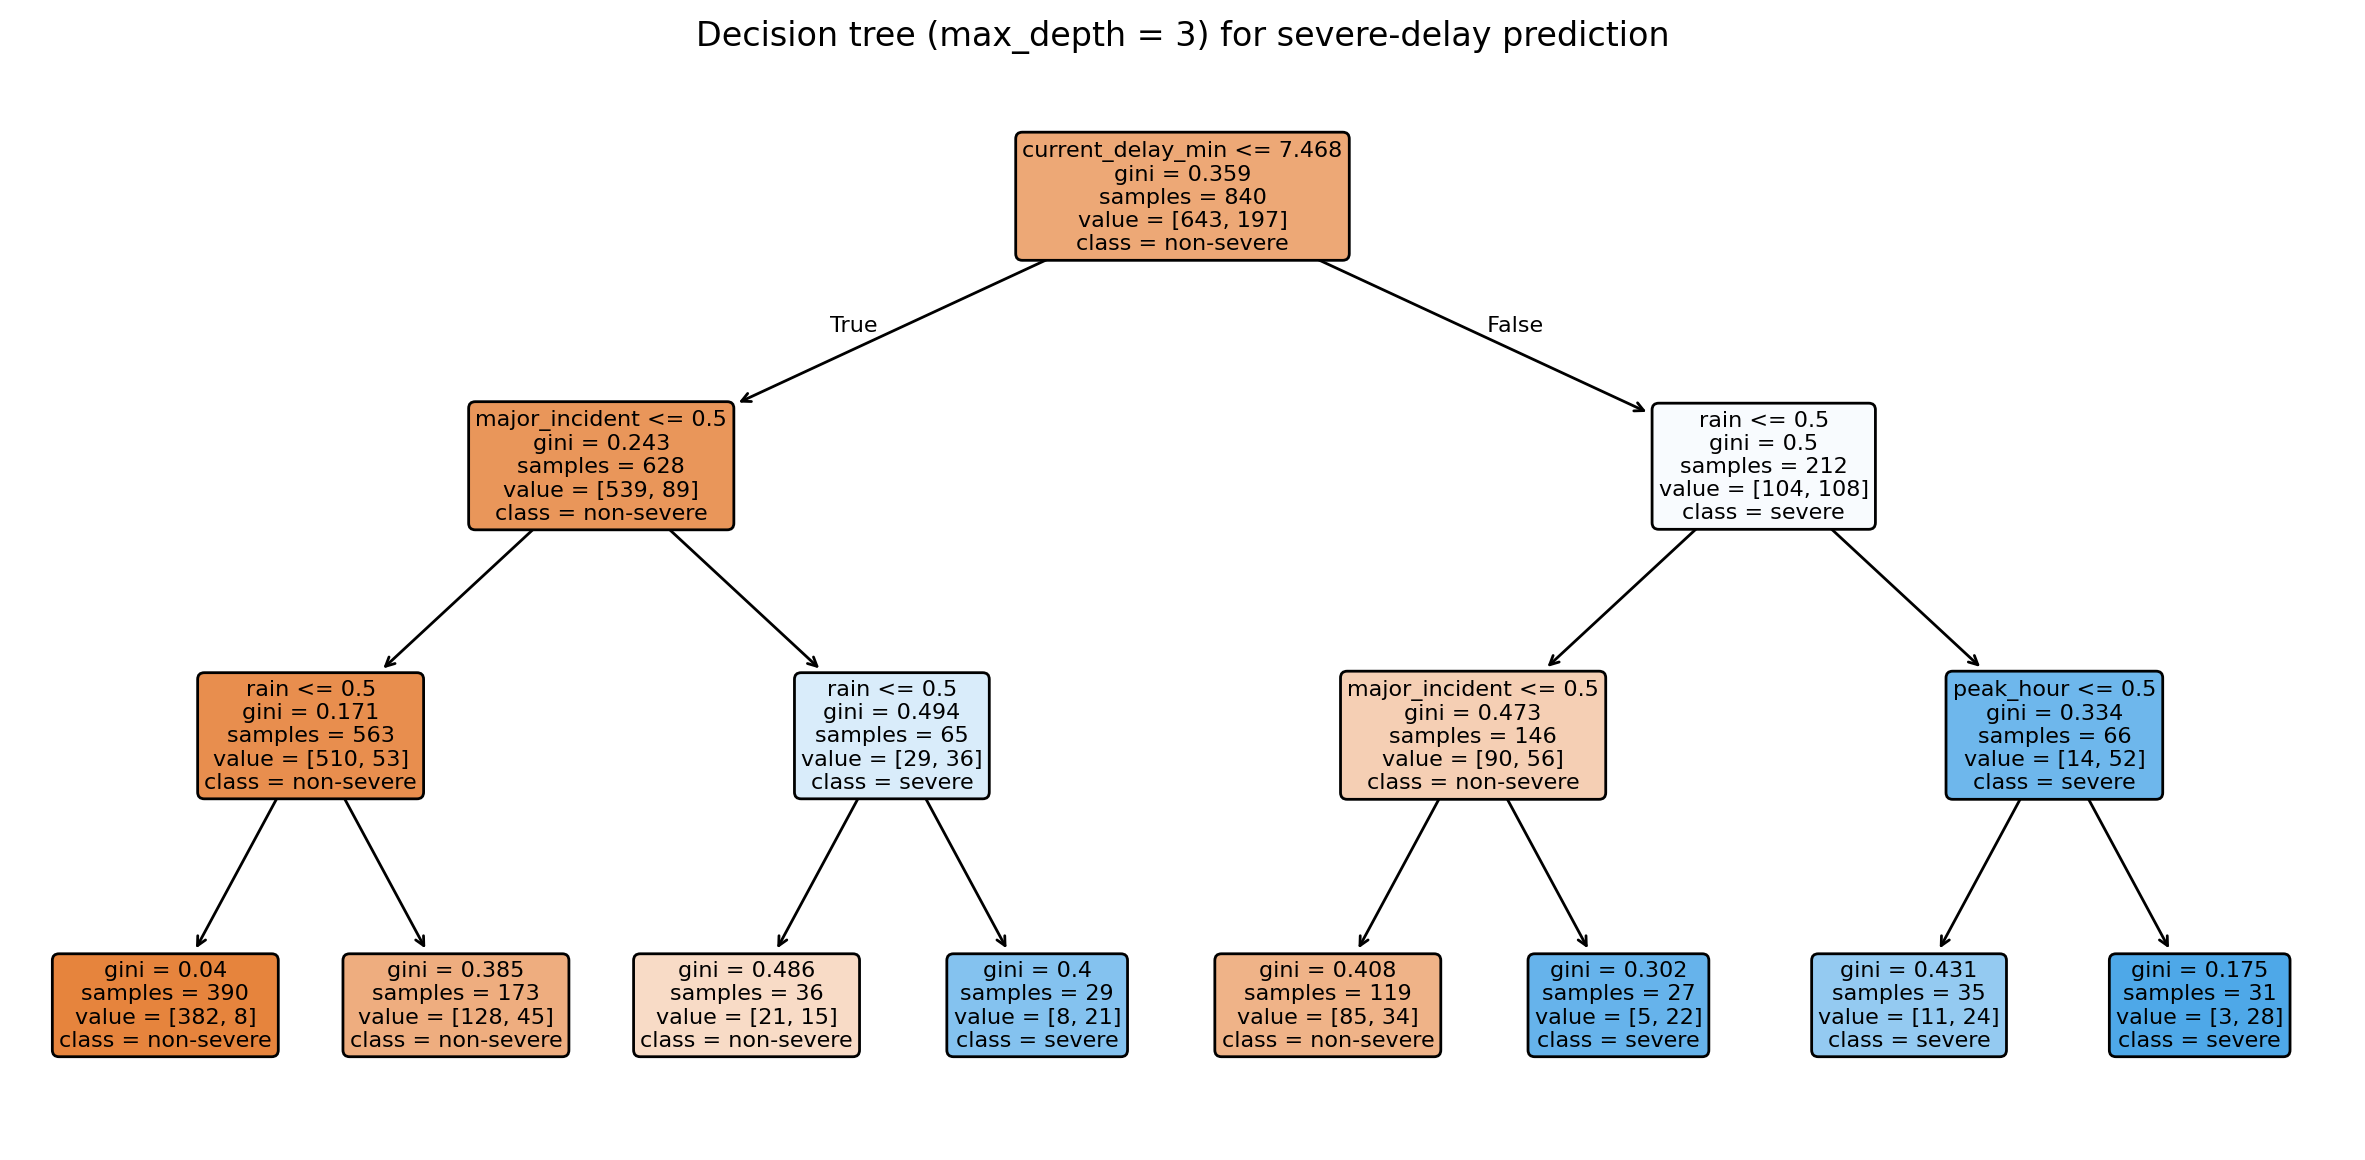
\includegraphics[width=\textwidth]{figures/p3_4_decision_tree.png}
\caption{The fitted decision tree with \code{max\_depth=3}.}
\label{fig:tree}
\end{figure}

\paragraph{Test-set performance.} Accuracy $0.8472$, F1-score $0.5600$, ROC-AUC $0.8469$,
and the confusion matrix
\[
\begin{pmatrix} 270 & 6 \\ 49 & 35 \end{pmatrix}
\quad\text{i.e.}\quad
\mathrm{TN}=270,\ \mathrm{FP}=6,\ \mathrm{FN}=49,\ \mathrm{TP}=35 .
\]
The tree has the highest precision of the three models ($0.8537$) but by far the lowest
recall ($0.4167$): it raises very few false alarms but misses 49 of the 84 severe delays in
the test set.

\subsubsection*{3.4.3 Comparison with random forest and gradient boosting (4 points)}

The random forest used \code{n\_estimators=300} and \code{min\_samples\_leaf=5}; the
gradient boosting classifier used \code{n\_estimators=150}, \code{learning\_rate=0.05} and
\code{max\_depth=3}. All three models were evaluated on the same 360 held-out incidents with
the same metrics. ROC-AUC was computed from predicted probabilities
(\code{predict\_proba}), not from hard labels. A majority-class baseline is included as a
reference point.

\begin{table}[H]
\centering
\caption{Test-set performance on 360 held-out incidents.}
\label{tab:metrics}
\footnotesize
\begin{tabular}{lrrrrrl}
\toprule
Model & Accuracy & Precision & Recall & F1-score & ROC-AUC & Confusion matrix \\
\midrule
Decision tree      & 0.8472 & \textbf{0.8537} & 0.4167 & 0.5600 & 0.8469 & $[[270, 6], [49, 35]]$ \\
Random forest      & 0.8528 & 0.7627 & 0.5357 & 0.6294 & \textbf{0.8972} & $[[262, 14], [39, 45]]$ \\
Gradient boosting  & \textbf{0.8583} & 0.7797 & \textbf{0.5476} & \textbf{0.6434} & 0.8810 & $[[263, 13], [38, 46]]$ \\
\midrule
Baseline (majority class) & 0.7667 & 0.0000 & 0.0000 & 0.0000 & 0.5000 & $[[276, 0], [84, 0]]$ \\
\bottomrule
\end{tabular}
\end{table}

\begin{figure}[H]
\centering
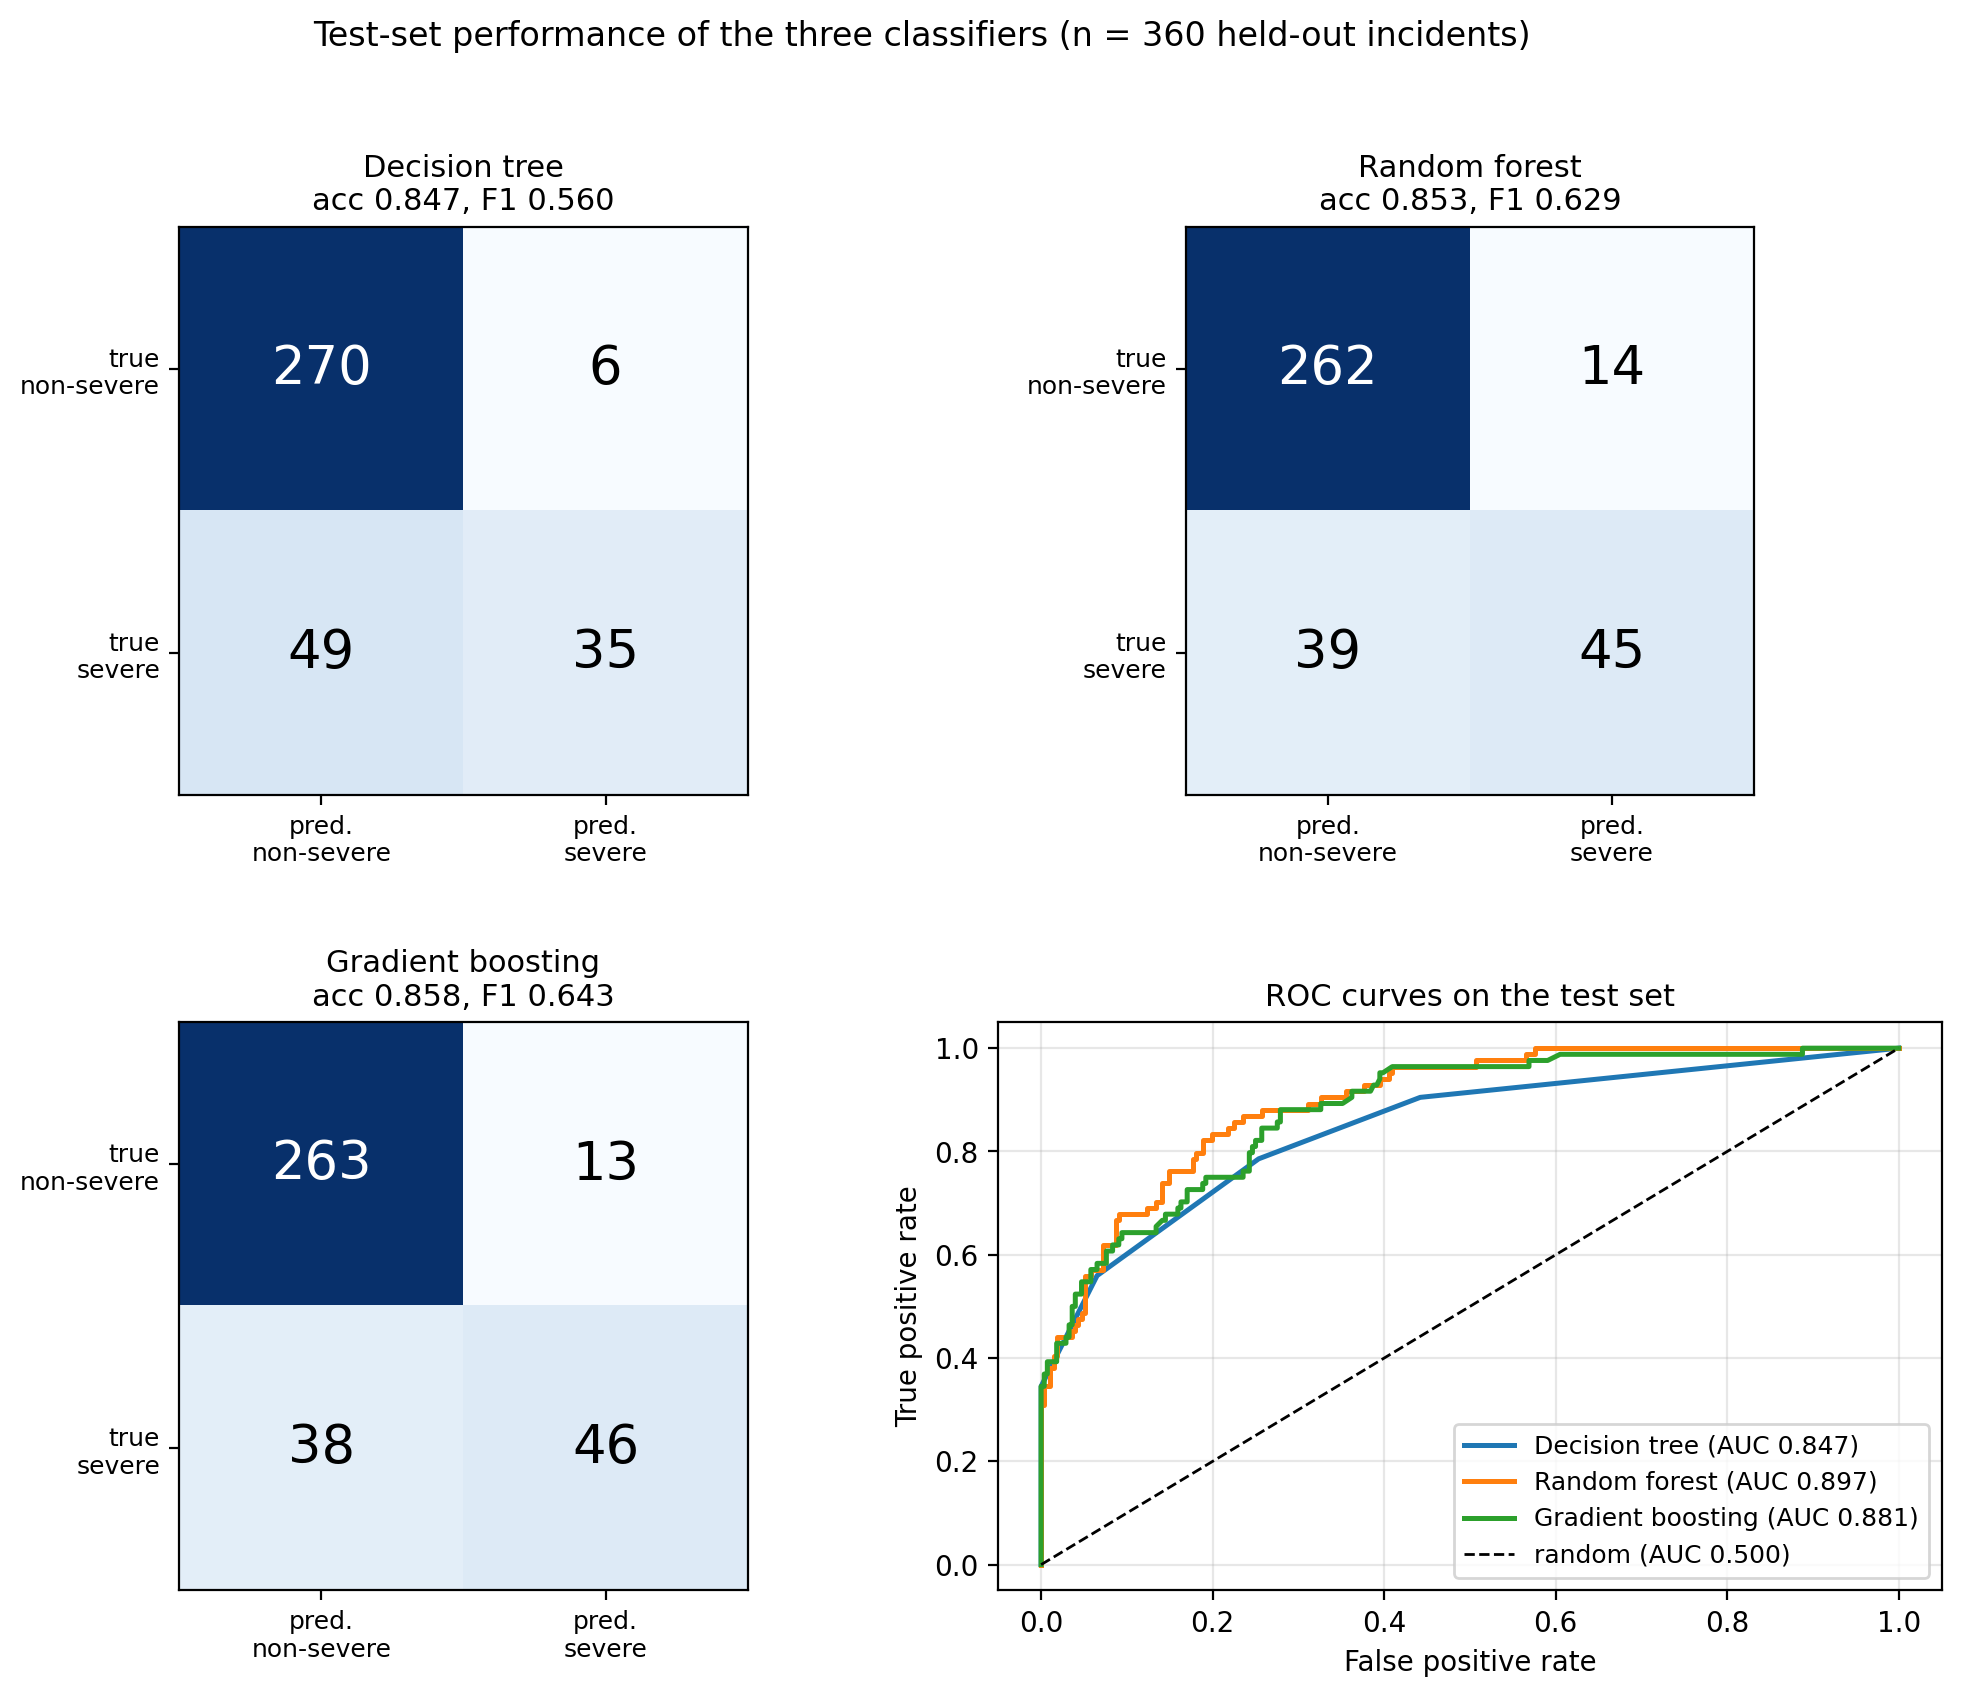
\includegraphics[width=0.82\textwidth]{figures/p3_4_confusion_and_roc.png}
\caption{Confusion matrices for the three models and their ROC curves on the test set.}
\label{fig:roc}
\end{figure}

To check that this ranking is not an artefact of one particular split, five-fold
cross-validated ROC-AUC was computed on the training data only:
decision tree $0.8535 \pm 0.0122$, random forest $0.9194 \pm 0.0093$, gradient boosting
$0.9141 \pm 0.0078$. The ordering is the same.

\paragraph{Interpretation.} Both ensembles clearly beat the single tree, and all three beat
the majority-class baseline --- the comparison that shows the models are doing real work
rather than exploiting the class imbalance. The ranking between the ensembles depends on the
metric: gradient boosting is best on accuracy and F1 at the default threshold, while the
random forest is best on ROC-AUC, which is threshold-independent and measures the quality of
the probability ranking rather than of any particular set of hard predictions.

The gains over the single tree arise from different mechanisms. The forest averages 300
decorrelated trees, which reduces variance; boosting fits 150 shallow trees sequentially to
the residuals with a learning rate of 0.05, which reduces bias. Both are better placed than
a depth-3 tree to represent the interaction terms in the generating process --- a tree of
depth 3 has only seven internal nodes with which to express six effects, several of them
interactions.

\subsubsection*{3.4.4 Feature importances (2 points)}

\begin{table}[H]
\centering
\caption{Impurity-based feature importances (each column sums to 1) and permutation
importance on the test set (mean drop in ROC-AUC over 30 shuffles).}
\label{tab:imp}
\begin{tabular}{lrrrcrrr}
\toprule
& \multicolumn{3}{c}{Impurity-based} & & \multicolumn{3}{c}{Permutation (test ROC-AUC drop)} \\
\cmidrule(lr){2-4}\cmidrule(lr){6-8}
Variable & Tree & Forest & Boosting & & Tree & Forest & Boosting \\
\midrule
\code{current\_delay\_min} & \textbf{0.3792} & \textbf{0.3741} & \textbf{0.3483} & & 0.1462 & 0.1353 & 0.1204 \\
\code{rain}                & 0.2801 & 0.1942 & 0.2141 & & 0.0605 & 0.0891 & 0.0787 \\
\code{major\_incident}     & 0.3269 & 0.1797 & 0.2101 & & 0.1448 & 0.1320 & 0.1181 \\
\code{passenger\_load}     & 0.0000 & 0.1474 & 0.1169 & & 0.0000 & 0.0412 & 0.0375 \\
\code{peak\_hour}          & 0.0138 & 0.0806 & 0.0906 & & 0.0035 & 0.0410 & 0.0445 \\
\code{critical\_hub}       & 0.0000 & 0.0240 & 0.0201 & & 0.0000 & 0.0153 & 0.0223 \\
\bottomrule
\end{tabular}
\end{table}

\begin{figure}[H]
\centering
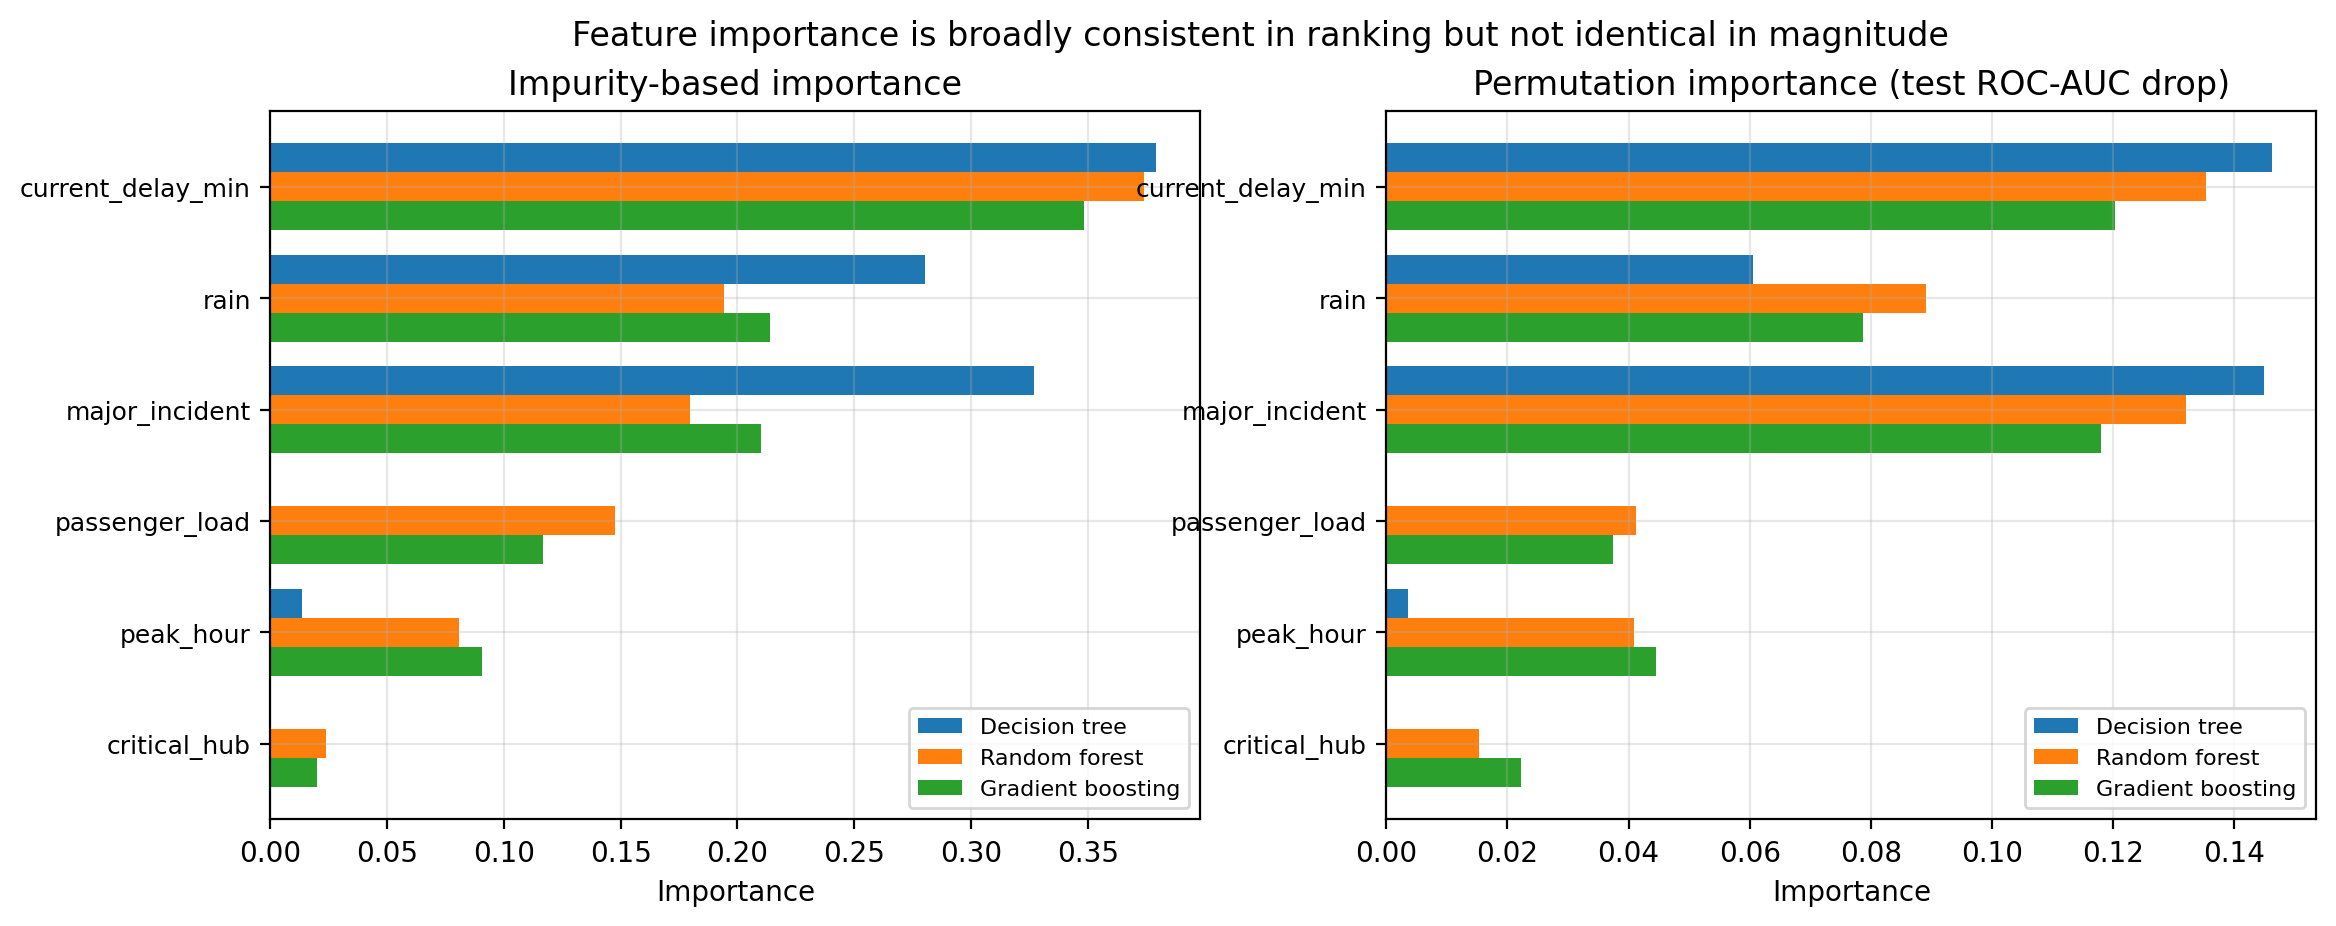
\includegraphics[width=\textwidth]{figures/p3_4_feature_importances.png}
\caption{Feature importance under both measures.}
\label{fig:imp}
\end{figure}

\paragraph{Which variables are most influential?} \code{current\_delay\_min} is the most
influential variable under the impurity measure in all three models ($0.3792$, $0.3741$,
$0.3483$), followed by \code{rain} and \code{major\_incident}. This matches the generating
process, in which the current delay enters two separate terms and \code{major\_incident}
carries the largest single coefficient of $1.5$.

\paragraph{Are the importances identical across methods?} \textbf{No}, and the differences
are informative. The depth-3 tree assigns exactly zero to \code{critical\_hub} and
\code{passenger\_load}, because with only seven splits available it never uses them; the
ensembles give \code{passenger\_load} a substantial $0.1474$ and $0.1169$ respectively.
Since \code{passenger\_load} appears in two interaction terms of the generating process, it
genuinely matters, so the tree's zero reflects its depth limit rather than irrelevance.
Conversely the tree over-weights \code{major\_incident} ($0.3269$) relative to the ensembles
($0.1797$ and $0.2101$).

Two general cautions apply. Impurity-based importance is biased towards continuous and
high-cardinality features: the two continuous variables here, \code{current\_delay\_min} and
\code{passenger\_load}, take 52\% of the total in the forest and 47\% in boosting, against
four binary variables sharing the remainder. And importances are shares constrained to sum
to one, so they measure relative rather than absolute contribution.

The permutation cross-check on the test set agrees on the top variable but narrows the gap
considerably: \code{current\_delay\_min} and \code{major\_incident} are almost tied in every
model ($0.1462$ versus $0.1448$ for the tree, $0.1353$ versus $0.1320$ for the forest,
$0.1204$ versus $0.1181$ for boosting). Because permutation importance is measured in units
of lost ROC-AUC on held-out data and is not biased towards continuous features, this
suggests the impurity measure was overstating the current delay's lead. The safer conclusion
is that the current delay and whether the incident is major are the two dominant predictors,
with rain third, rather than that there is a single clear winner.

\subsubsection*{3.4.5 Recommendation and the false positive / false negative trade-off (2 points)}

\paragraph{Recommendation.} I recommend the \textbf{random forest}, while noting that the
choice is close and depends on how the tool would be used.

The case rests on ROC-AUC ($0.8972$, against $0.8810$ for boosting and $0.8469$ for the
tree), a margin confirmed by cross-validation on the training data. A control centre would
not consume hard $0/1$ predictions; it would rank live incidents by predicted severity and
act on the top of the list, and ROC-AUC measures exactly that ranking quality independently
of any threshold. The forest also requires less tuning than boosting, provides out-of-bag
error estimates at no extra cost, and is more robust to its hyperparameters being somewhat
wrong --- all of which matter for a model that has to be maintained in operational service.

If instead the tool were to issue automatic binary alerts at a fixed threshold, gradient
boosting's higher F1-score ($0.6434$) would make it the better choice. The single tree
should not be deployed for prediction despite being the most transparent of the three, but
it retains value as an explanation aid, since a depth-3 tree fits on one page and can be
shown directly to controllers.

\paragraph{The trade-off between false positives and false negatives.} This is the more
consequential decision. At the default threshold of 0.5 the random forest produces 14 false
positives and 39 false negatives out of 360 test incidents. The two errors are not equally
costly:

\begin{itemize}[leftmargin=2em]
\item A \textbf{false positive} means staff are placed on standby or passengers are warned
about a delay that does not materialise. The cost is wasted resource and, if it recurs,
alert fatigue that erodes controllers' trust in the system.
\item A \textbf{false negative} means a severe delay develops with no warning, so no
replacement service is arranged and no passenger information is issued. The cost falls on
passengers and on the operator's punctuality record, and it is generally the larger of the
two.
\end{itemize}

Given that asymmetry, missing 39 of 84 severe delays (recall $0.5357$) is difficult to
defend, and the default threshold of 0.5 is a software convention rather than a property of
the model.

\paragraph{Selecting the threshold without touching the test set.} Choosing a threshold is
a model-selection decision, so it must not be made on the test data. I therefore follow a
four-step protocol:

\begin{enumerate}[leftmargin=2em]
\item generate out-of-fold probabilities for the training set using five-fold stratified
cross-validation, so that every training row is scored by a model that did not see it;
\item sweep the threshold on those out-of-fold probabilities and select the F1-maximising
value (Figure~\ref{fig:thresh});
\item refit on the full training set;
\item apply the selected threshold to the test set \textbf{once}, as a final evaluation.
\end{enumerate}

The out-of-fold ROC-AUC is $0.9147$ and the selected threshold is $\mathbf{0.440}$, with an
out-of-fold F1 of $0.7301$. Table~\ref{tab:thresh} reports what that threshold then does on
the test set.

\begin{figure}[H]
\centering
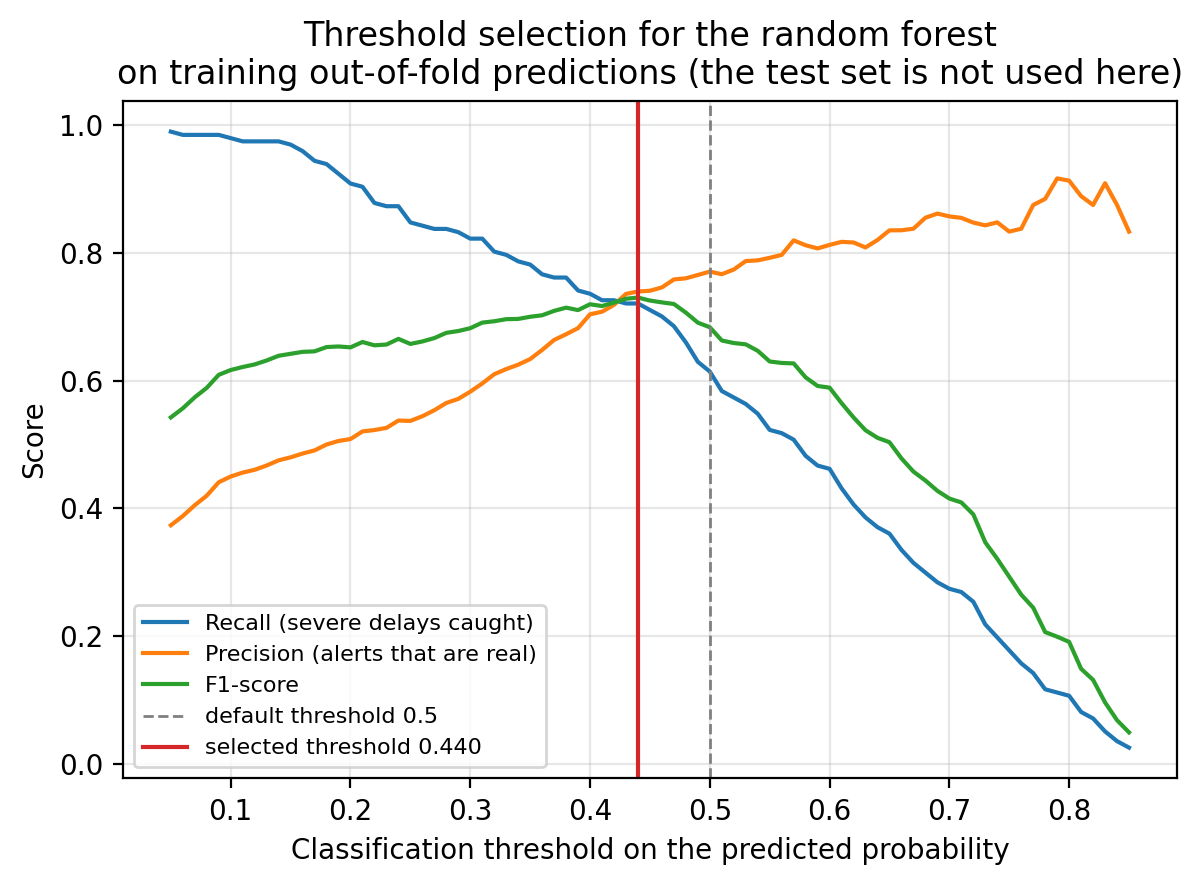
\includegraphics[width=0.62\textwidth]{figures/p3_4_threshold_tradeoff.png}
\caption{Threshold selection for the random forest on training out-of-fold predictions. The
test set plays no part in this figure.}
\label{fig:thresh}
\end{figure}

\begin{table}[H]
\centering
\caption{Test-set performance of the threshold selected on training data, evaluated once on
the 360 held-out incidents.}
\label{tab:thresh}
\begin{tabular}{lrrrrr}
\toprule
Threshold & Recall & Precision & F1-score & False positives & False negatives \\
\midrule
0.500 (default)  & 0.5357 & 0.7627 & 0.6294 & 14 & 39 \\
0.440 (selected) & 0.5952 & 0.7143 & 0.6494 & 20 & 34 \\
\bottomrule
\end{tabular}
\end{table}

The selected threshold raises recall from $0.5357$ to $0.5952$, cutting missed severe delays
from 39 to 34, while false alarms rise from 14 to 20; test F1 improves from $0.6294$ to
$0.6494$.

The modest size of that gain is itself worth reporting. A threshold tuned directly on the
test set would appear to do considerably better, but that appearance would be partly an
artefact of fitting noise in 360 observations, and it would not carry over to new incidents.
Selecting on out-of-fold training predictions yields a smaller but honest estimate of field
performance and preserves the test set as a genuine held-out sample. The practical
implication for the control centre is that if recall substantially above $0.6$ is required,
the answer is not a more aggressive threshold but a better model or more informative
features.

Finally, F1 is only a stand-in for the operator's real objective, since it weights precision
and recall equally --- precisely the assumption argued against above. In practice the
threshold should minimise expected cost,
$C_{\mathrm{FN}}\cdot \mathrm{FN} + C_{\mathrm{FP}}\cdot \mathrm{FP}$, using the operator's
own estimates of the two costs. The same out-of-fold procedure applies unchanged, with that
cost function replacing F1 as the selection criterion.

\paragraph{Assumptions and limitations.} The dataset is synthetic and generated from a known
additive score, so these results indicate how well each method recovers a structure of that
particular kind; they are not evidence about real incident data, which would bring
measurement error, temporal correlation between incidents, non-stationarity as the network
and timetable change, and covariates not recorded here. The test set contains 360
observations, so the metrics carry meaningful sampling uncertainty --- a difference of one
or two points in accuracy between the forest and boosting is within noise, which is why the
cross-validated results were used as corroboration. Finally, the features are operational
correlates of severe delay, not causes. The models support prediction and prioritisation,
and they do not license conclusions about what would happen if an intervention changed one
of these variables.

\end{document}
